\documentclass[12pt,a4paper]{report}

% Packages
\usepackage{geometry}
\usepackage{amsmath}
\usepackage{amsfonts}
\usepackage{amssymb}
\usepackage{graphicx}
\usepackage{listings} % for code listing
\usepackage{subcaption}
\usepackage{tabularx}
\usepackage{hyperref}
\usepackage{wrapfig}

% Geometry
\geometry{a4paper, margin=1in}

% Title
\title{Computer Vision Homework Report \\ \Large Homework 2}

\author{Chinatip Lawansuk\\\\112998405}
\date{}


% For code listings
\lstset{
  basicstyle=\ttfamily\small,
  breaklines=true,
  frame=single,
  language=C++  % this line sets the language to C++
}

\begin{document}

\maketitle

\tableofcontents

\chapter{Introduction}
This project focuses on develop an algorithm to perform principle operations in Computer Vision from scratch.

\section{Objectives}
\begin{enumerate}
  \item Understand Theory of Computer Vision
  \item Improve C++/Python Programming Skill
\end{enumerate}

\section{Requirements}
\begin{enumerate}
  \item Write a Mean filter operation (customise kernel size and padding independently).
  \item Write a Median filter operation (customise kernel size and padding independently).
  \item Show the Histogram for both original images and processed images
\end{enumerate}

\section{System Configuration}
\subsection{Hardware}
\begin{itemize}
  \item CPU\@: Intel Core-i7
  \item GPU\@: NVIDIA
  \item RAM\@: 40 GB
\end{itemize}

\subsection{Software}
\begin{itemize}
  \item OS\@: Windows Subsystem Linux x64 (Ubuntu 22.04.3 LTS Kernel Ver. 5.15.90.1)
  \item GCC Version\@: \verb|11.4.0 x86_64-linux-gnu|
  \item OpenCV Version\@: \verb|4.5.4+dfsg-9ubuntu4|
\end{itemize}

\chapter{Solution, Explanation, and Result}
In this project, code explanation is embedded in the comment section in the code.

\section{Main Function}
The main function of the program will load the desired picture, apply the function sequentially, display on the window, and write a new file for the proceeded image.
\begin{lstlisting}
#include <stdio.h>
#include <opencv2/opencv.hpp>
#include <unistd.h>
#include <string.h>
#include "include/func.hpp"

#define MAX_LEN 250
#define BASE_PATH "/home/chinatip/work/computer_vision/homework2"
#define SRC_PATH "test_img"
#define OUT_PATH "output"

// define file name, can uncomment to select the input
#define FILENAME "noise1"
// #define FILENAME "noise2"
#define MEAN_FILT_SUFX "q1"
#define MEDIAN_FILT_SUFX "q2"
#define KER_INFO_3 "K3P1"
#define KER_INFO_5 "K5P2"
#define KER_INFO_7 "K7P3"
#define EXT "png"

using namespace cv;

Mat canvas;

void appendImgToCanvas(Mat);

int main(int argc, char **argv)
{

    Mat og_img;
    char og_file[MAX_LEN] = "", out_file[MAX_LEN] = "";
    snprintf(og_file, MAX_LEN, "%s/%s/%s.%s", BASE_PATH, SRC_PATH, FILENAME, EXT);

    og_img = imread(og_file);

    if (!og_img.data)
    {
        printf("No image data \n");
        return -1;
    }
    else
    {
        printf("Original Img Size: w x h %d x %d\n", og_img.cols, og_img.rows);
    }

    appendImgToCanvas(og_img);

    Mat res_img;
    res_img = applyMedianFilter(og_img,3,1,1);
    printf("Median Filter Img Size: w x h %d x %d\n", res_img.cols, res_img.rows);
    snprintf(out_file, MAX_LEN, "%s/%s/%s_%s.%s", BASE_PATH, OUT_PATH, FILENAME, MEDIAN_FILT_SUFX, EXT);
    imwrite(out_file, res_img);
    snprintf(out_file, MAX_LEN, "%s/%s/%s_%s_%s.%s", BASE_PATH, OUT_PATH, FILENAME, MEDIAN_FILT_SUFX,KER_INFO_3, EXT);
    imwrite(out_file, res_img);
    appendImgToCanvas(res_img);

    res_img = applyMedianFilter(og_img,5,2,1);
    printf("Median Filter Img Size: w x h %d x %d\n", res_img.cols, res_img.rows);
    snprintf(out_file, MAX_LEN, "%s/%s/%s_%s_%s.%s", BASE_PATH, OUT_PATH, FILENAME, MEDIAN_FILT_SUFX,KER_INFO_5, EXT);
    imwrite(out_file, res_img);
    appendImgToCanvas(res_img);

    res_img = applyMedianFilter(og_img,7,3,1);
    printf("Median Filter Img Size: w x h %d x %d\n", res_img.cols, res_img.rows);
    snprintf(out_file, MAX_LEN, "%s/%s/%s_%s_%s.%s", BASE_PATH, OUT_PATH, FILENAME, MEDIAN_FILT_SUFX,KER_INFO_7, EXT);
    imwrite(out_file, res_img);
    appendImgToCanvas(res_img);

    namedWindow("Original", WINDOW_AUTOSIZE);
    
    imshow("Original", canvas);
    waitKey(0);
    return 0;
}

void appendImgToCanvas(Mat img)
{
    if (canvas.empty())
    {
        canvas = img;
    }
    else
    {
        Size s(canvas.cols + img.cols + 5, canvas.rows>img.rows?canvas.rows:img.rows);
        size_t old_w = canvas.cols;
        copyMakeBorder(canvas, canvas, 0, 0, 0, img.cols + 5, BORDER_CONSTANT, Scalar(0, 0, 0, 0));
        img.copyTo(canvas(Rect(old_w + 5, 0, img.cols, img.rows)));
    }
}

\end{lstlisting}
\begin{figure}[!htb]
  \centering
  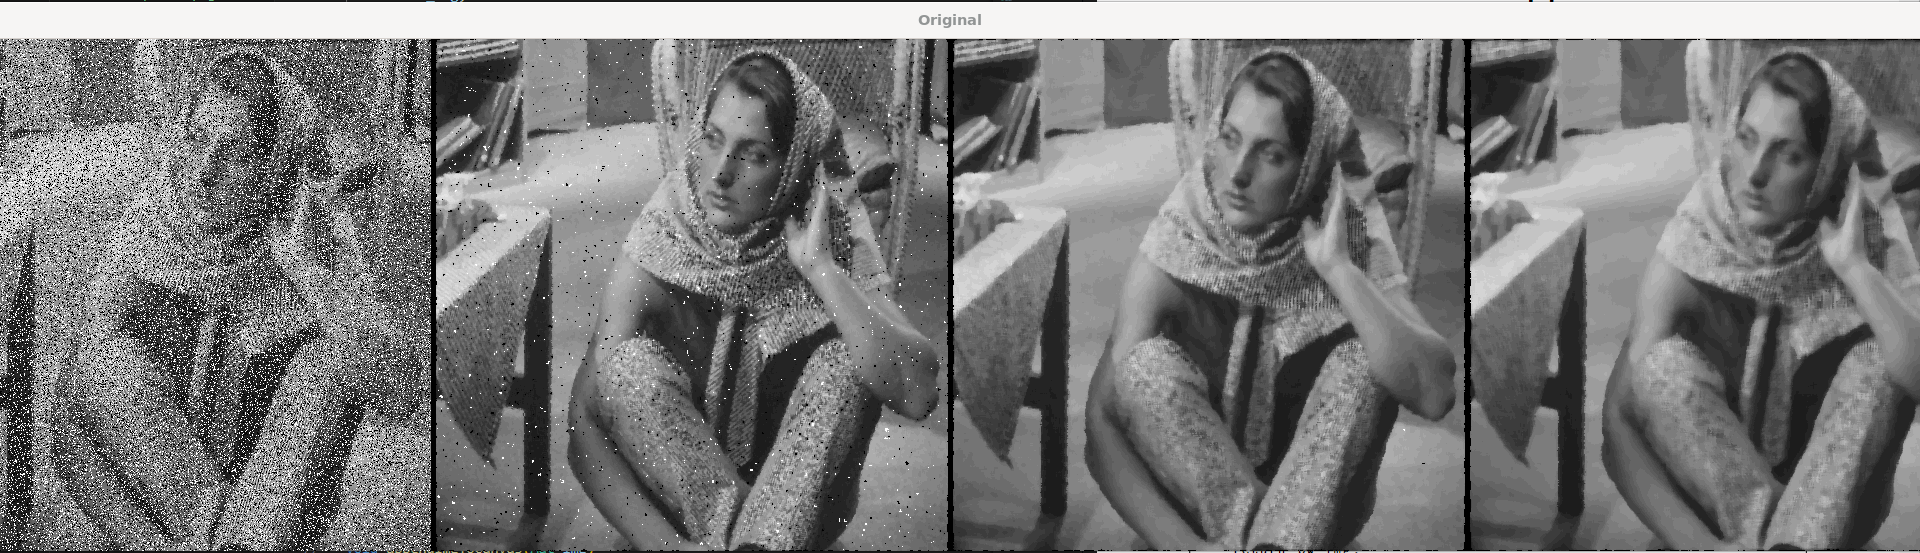
\includegraphics[width=1\linewidth]{program.png}
  \caption{Program Output (Automatic place image in frame)}
\end{figure}
\clearpage


\section{Applying Mean Filter}
\begin{tabular}{lll}
  Input  & : & Matrix of Input Image  \\
         &   & Kernel size (Integer)  \\
         &   & Padding size (Integer)  \\
         &   & Stride size (Integer)  \\
  Output & : & Matrix of Output Image \\
\end{tabular}
\begin{lstlisting}
Mat applyMeanFilter (Mat img, int kernel_size, int padding, int stride)
{
  // calculate kernel offset ie. number of pixel before and 
  // after since the target pixel will be the center of 
  // matrix,
  // in order to get the neighbour pixel with size of kernel
  // size, offset will be applied for both before, and after
  // the target pixel
  // example
  // width = 5 => offset = (int)5/2 = 2;
  // px   ... k   n-offset    ... n   ... n+offset    k
  int ker_x_offset = kernel_size / 2;
  int ker_y_offset = kernel_size / 2;

  // get kernel size
  int ker_w = kernel_size;
  int ker_h = kernel_size;

  // calculate output image size
  int out_w = ((img.cols + (2 * padding) - kernel_size) / stride) + 1;
  int out_h = ((img.rows + (2 * padding) - kernel_size) / stride) + 1;

  // create intermediate buffer and add padding, size is 
  // w+(2*padding),h+(2*padding) then copy the content 
  // of image to the buffer
  Mat padded;
  padded = Mat::zeros(img.rows + (2 * padding), img.cols + (2 * padding), CV_32SC3);
  for (int j = 0; j < img.rows; j++)
  {
      for (int i = 0; i < img.cols; i++)
      {
          padded.at<Vec3i>(j+padding,i+padding)=img.at<Vec3b>(j,i);
      }
  }
  
  // create output buffer with calculated output size
  // data type need to be vector of signed int 32 bit
  // in case negative data is possible, this can help
  // preserve information through the convolution process
  // and rasterise to 8 bit at the last step
  Mat img_res = Mat::zeros(out_h, out_w, CV_32SC3);
  Vec3i res(0, 0, 0);
  Point2i start=Point2i(0,0);

  // iterate over the size of output image
  for (int out_j = 0; out_j < out_h; out_j++)
  {
      for (int out_i = 0; out_i < out_w; out_i++)
      {
          
          // calculate the start point to slice a windowed from 
          // the padded buffer
          start.x=(out_i*stride)+padding-ker_x_offset;
          start.y=(out_j*stride)+padding-ker_x_offset;

          // get windowed matrix from the padded buffer with 
          // the size of kernel size, and target pixel is in
          // the center of windowed matrix
          Mat windowed = padded(Rect(start.x, start.y, ker_w, ker_h));
          res = Vec3i(0, 0, 0);


          // accumulate each pixel in window
          for (int ker_j = 0; ker_j < kernel_size; ker_j++)
          {
              for (int ker_i = 0; ker_i < kernel_size; ker_i++)
              {
                  Vec3b t = windowed.at<Vec3i>(ker_i, ker_j);
                  
                  // add to buffer
                  res+=t;
              }
          }

          for (int c = 0; c < 3; c++)
          {
              // divide by the number of elements to get the 
              // average
              res[c] /= (kernel_size*kernel_size);
          }

          // write to output buffer
          img_res.at<Vec3i>(out_j,out_i) = res;
      }
  }
  // return the output image
  return img_res;
}
\end{lstlisting}
\begin{figure}[!htb]
  \centering
  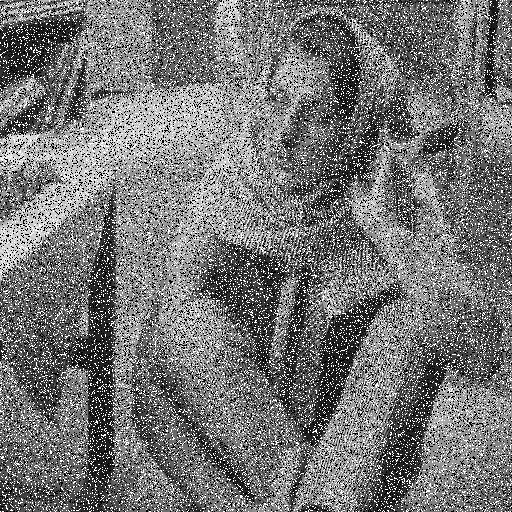
\includegraphics[height=0.4\paperheight]{test_img/noise1.png}
  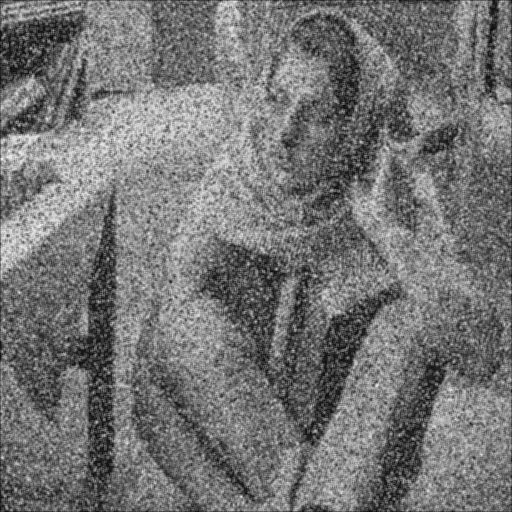
\includegraphics[height=0.4\paperheight]{result_img/noise1_q1.png}
  \caption{Comparison Between (U) Original and (L) Mean Filter Applied Kernel=3, Padding=1}
\end{figure}
\clearpage

\section{Apply Median}
\begin{tabular}{lll}
  Input  & : & Matrix of Input Image  \\
         &   & Kernel size (Integer)  \\
         &   & Padding size (Integer)  \\
         &   & Stride size (Integer)  \\
  Output & : & Matrix of Output Image \\
\end{tabular}
\begin{lstlisting}
Mat applyMedianFilter (Mat img, int kernel_size, int padding, int stride)
{
  // calculate kernel offset ie. number of pixel before and 
  // after since the target pixel will be the center of 
  // matrix,
  // in order to get the neighbour pixel with size of kernel
  // size, offset will be applied for both before, and after
  // the target pixel
  // example
  // width = 5 => offset = (int)5/2 = 2;
  // px   ... k   n-offset    ... n   ... n+offset    k
  int ker_x_offset = kernel_size / 2;
  int ker_y_offset = kernel_size / 2;

  // get kernel size
  int ker_w = kernel_size;
  int ker_h = kernel_size;

  // calculate output image size
  int out_w = ((img.cols + (2 * padding) - kernel_size) / stride) + 1;
  int out_h = ((img.rows + (2 * padding) - kernel_size) / stride) + 1;

  // create intermediate buffer and add padding, size is 
  // w+(2*padding),h+(2*padding) then copy the content 
  // of image to the buffer
  Mat padded;
  padded = Mat::zeros(img.rows + (2 * padding), img.cols + (2 * padding), CV_32SC3);
  for (int j = 0; j < img.rows; j++)
  {
      for (int i = 0; i < img.cols; i++)
      {
          padded.at<Vec3i>(j+padding,i+padding)=img.at<Vec3b>(j,i);
      }
  }
  
  // create output buffer with calculated output size
  // data type need to be vector of signed int 32 bit
  // in case negative data is possible, this can help
  // preserve information through the convolution process
  // and rasterise to 8 bit at the last step
  Mat img_res = Mat::zeros(out_h, out_w, CV_32SC3);
  Vec3i res(0, 0, 0);
  Point2i start=Point2i(0,0);

  // iterate over the size of output image
  for (int out_j = 0; out_j < out_h; out_j++)
  {
      for (int out_i = 0; out_i < out_w; out_i++)
      {

          
          // calculate the start point to slice a windowed from 
          // the padded buffer
          start.x=(out_i*stride)+padding-ker_x_offset;
          start.y=(out_j*stride)+padding-ker_x_offset;

          // get windowed matrix from the padded buffer with 
          // the size of kernel size, and target pixel is in
          // the center of windowed matrix
          Mat windowed = padded(Rect(start.x, start.y, ker_w, ker_h));
          res = Vec3i(0, 0, 0);

          // create buffer lists for each channel
          std::vector<int32_t> b,g,r;


          // item-wise split channel data             
          for (int ker_j = 0; ker_j < kernel_size; ker_j++)
          {
              for (int ker_i = 0; ker_i < kernel_size; ker_i++)
              {
                  Vec3b t = windowed.at<Vec3i>(ker_i, ker_j);
              
                  // add each channel to its buffer list
                  b.push_back(t[0]);
                  g.push_back(t[1]);
                  r.push_back(t[2]);
              }
          }
          
          // apply sort function to each channel
          b=sort(b);
          r=sort(r);
          g=sort(g);

          // get the median ie. the middle item of the list
          // as a representative for each window
          int idx=b.size()/2;
          res[0]=b.at(idx);
          res[1]=g.at(idx);
          res[2]=r.at(idx);

          // write to output buffer
          img_res.at<Vec3i>(out_j,out_i) = res;
          
      }
  }

  // return the output image
  return img_res;
}

// Sorting Algorithm: Insertion Sort Using Linked List

// Define Node Structure
typedef struct node
{
  int32_t val;
  struct node* next;
  bool is_term;
}node_t;

// Define End node
node_t END={.val=0,.next=nullptr,.is_term=true};

std::vector<int32_t> sort(std::vector<int32_t> list){
  // using insertion sort

  // initialise head of the list, and point to the end
  node_t head={.next=&END};
  node_t* cur;
  node_t* tmp;

  // for each item in list
  for(int i=0;i<list.size();i++){

      // first, set current node to head
      cur=&head;

      // create new node with current data
      tmp=(node_t*)malloc(sizeof(node_t));
      tmp->val=list.at(i);

      // traverse through linked list
      while(true){
          if(cur->next->is_term==true){

              // if reach end node, insert new node as
              // the last node of the linked list
              tmp->next=cur->next;
              cur->next=tmp;
              break;
          }
          else if(tmp->val<=cur->next->val){

              // if not the last node, compare value with
              // the next node, if lesser or equal to the 
              // next node, put new node at the current 
              // position and point to the next
              tmp->next=cur->next;
              cur->next=tmp;
              break;
          }

          // else, continue to next node
          cur=cur->next;
      }
  }

  // after sort, traverse through linked list and put back 
  // to vector
  cur=&head;
  cur=cur->next;
  std::vector<int32_t> res;
  while(!cur->is_term){
      res.push_back(cur->val);
      tmp=cur;
      cur=cur->next;
      free(tmp);
  }

  // return result
  return res;
}
\end{lstlisting}
\begin{figure}[!htb]
  \centering
  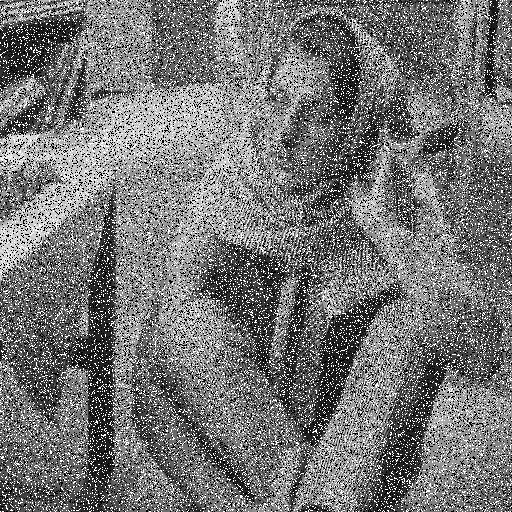
\includegraphics[height=0.4\paperheight]{test_img/noise1.png}
  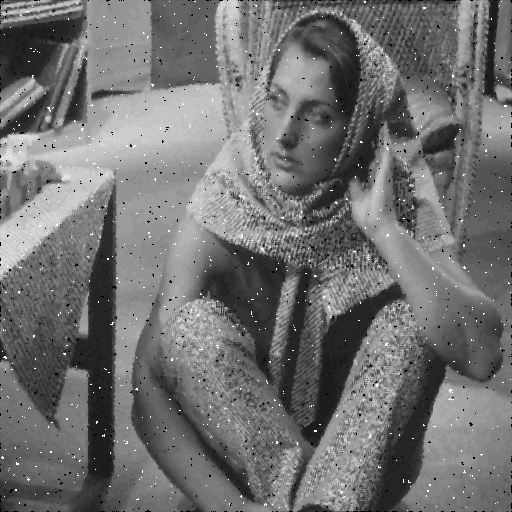
\includegraphics[height=0.4\paperheight]{result_img/noise1_q2.png}
  \caption{Comparison Between (U) Original and (L) Median Filter Applied Kernel=3, Padding=1}
\end{figure}
\clearpage


\chapter{Discussion}
\section{Observations}
\subsection{Kernel size affect in Mean Filter}
\paragraph*{}
Selecting lower number of kernel size means lower number of sampling group hence, if noise densely distributed in some area or the noise value is spiked, the mean filter might can not overcome the noise due to lacking of information.
\paragraph*{}One of effect that need to be mentioned is the mean filter reduces edge sharpness. Since it calculates by average over the area, when gradually shifts, the high-difference area (which is tends to be edge) gradually move on the window, and get avaraged every time. Resulting in loss of edge sharpness.
On the other hand, selecting higher number of kernel size tends to make the result lost its `locality' since it has information of points that may be too far from considered point. 
\paragraph*{}Mean filter smoothen the histogram curve, as shown in Figure~\ref{fig:n1-mean-hist} and ~\ref{fig:n2-mean-hist}.

\begin{figure}[!htb]
  \begin{minipage}{\linewidth}
    \centering
    \begin{subfigure}{0.49\textwidth}
      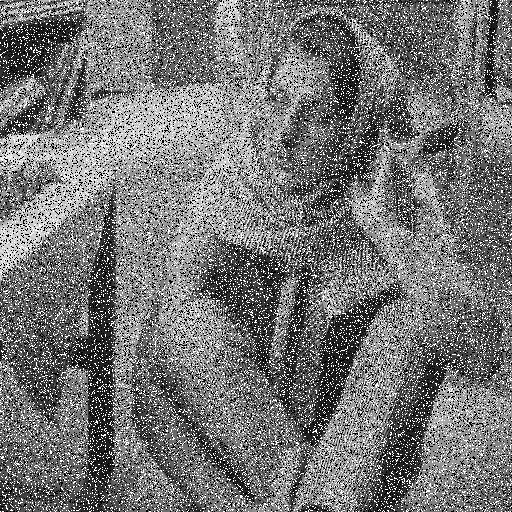
\includegraphics[width=\linewidth]{test_img/noise1.png}
      \subcaption{Original Image}
    \end{subfigure}
    \begin{subfigure}{0.49\textwidth}
      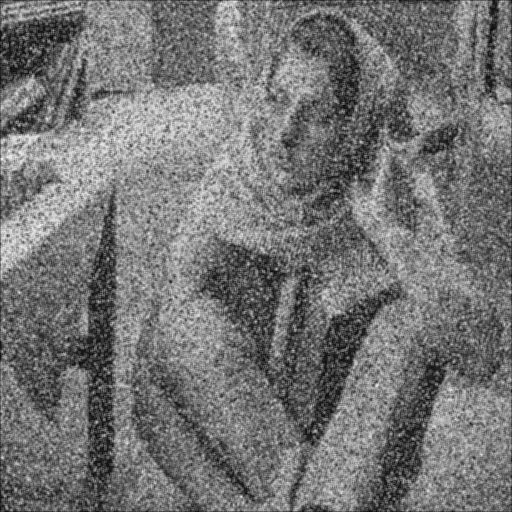
\includegraphics[width=\linewidth]{output/noise1_q1_K3P1.png}
    \subcaption{Kernel = 3}
    \end{subfigure}

    \begin{subfigure}{0.49\textwidth}
      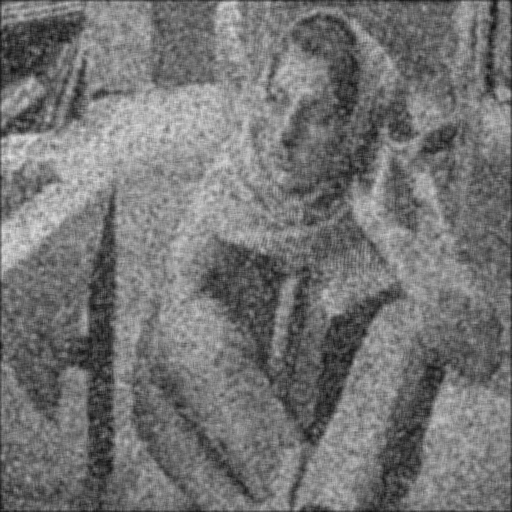
\includegraphics[width=\linewidth]{output/noise1_q1_K5P2.png}
    \subcaption{Kernel = 5}
    \end{subfigure}
    \begin{subfigure}{0.49\textwidth}
      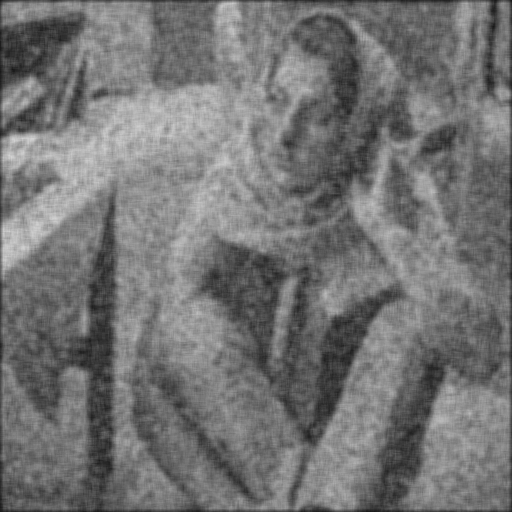
\includegraphics[width=\linewidth]{output/noise1_q1_K7P3.png}
    \subcaption{Kernel = 7}
    \end{subfigure}

  \caption{Comparison of noise1.png using Mean filter on different kernel size}
  \end{minipage}

\end{figure}
\begin{figure}[!htb]
  \begin{minipage}{\linewidth}
    \centering
    \begin{subfigure}{1\textwidth}
      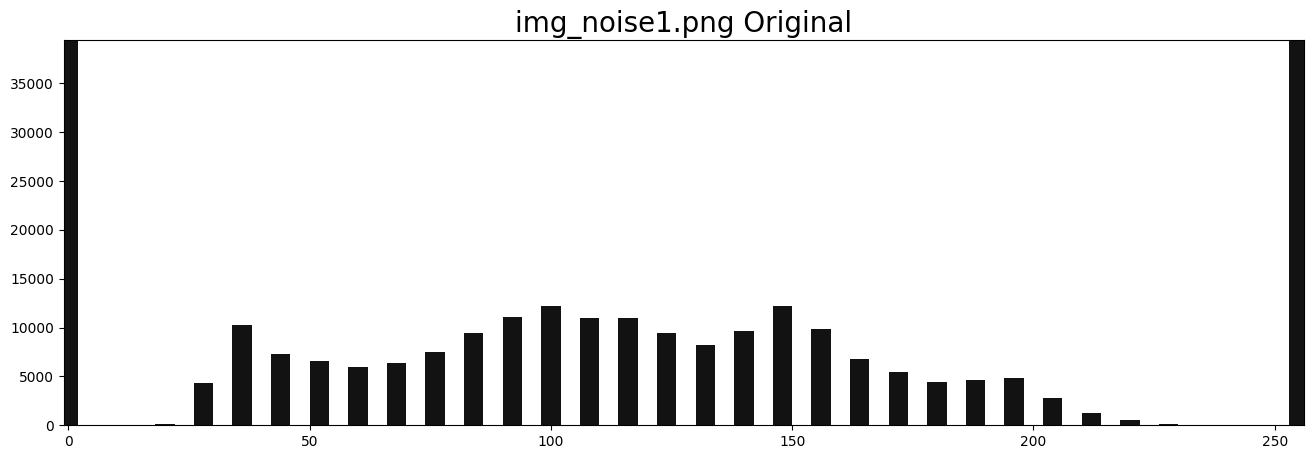
\includegraphics[height=5.3cm]{result_img/noise1_his.png}
      \subcaption{Original Image}
    \end{subfigure}
    \begin{subfigure}{1\textwidth}
      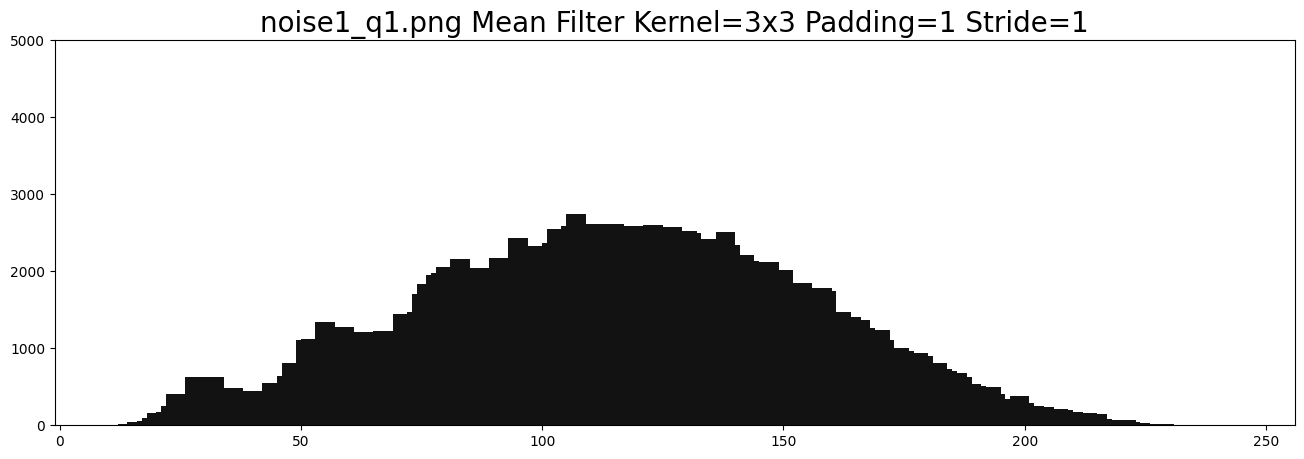
\includegraphics[height=5.3cm]{output/noise1_q1_K3P1_his.png}
    \subcaption{Kernel = 3}
    \end{subfigure}

    \begin{subfigure}{1\textwidth}
      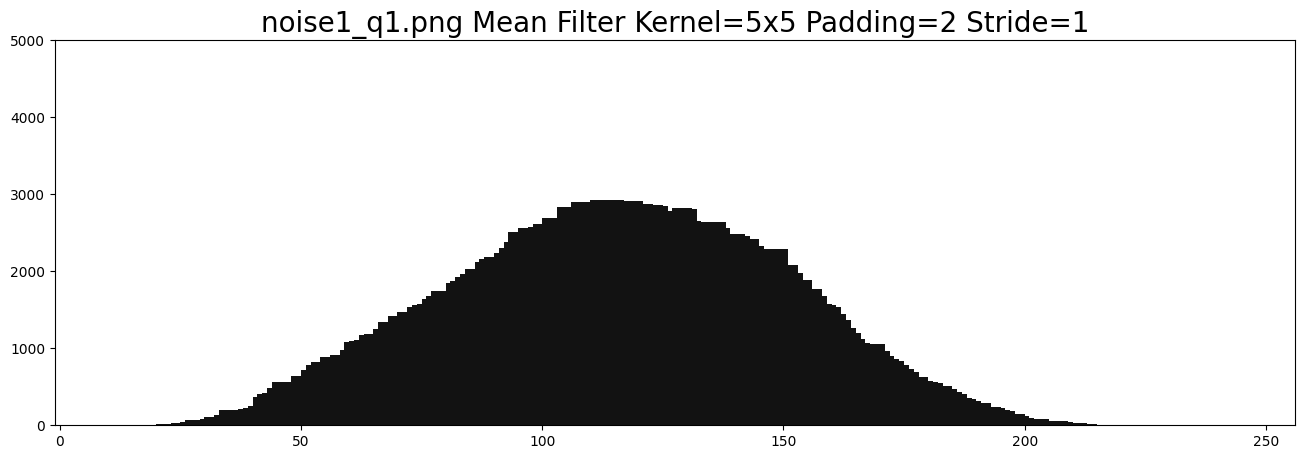
\includegraphics[height=5.3cm]{output/noise1_q1_K5P2_his.png}
    \subcaption{Kernel = 5}
    \end{subfigure}
    \begin{subfigure}{1\textwidth}
      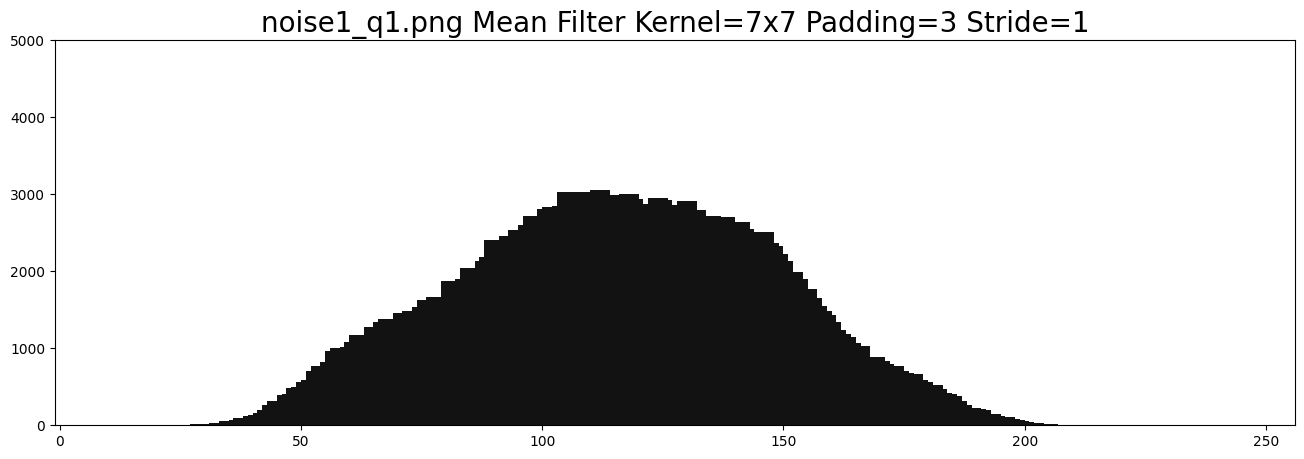
\includegraphics[height=5.3cm]{output/noise1_q1_K7P3_his.png}
    \subcaption{Kernel = 7}
    \end{subfigure}
    
  \caption{Comparison of Histogram of noise1.png using Mean filter on different kernel size}
\label{fig:n1-mean-hist}
\end{minipage}
\end{figure}
\begin{figure}[!htb]
  \begin{minipage}{\linewidth}
    \centering
    \begin{subfigure}{0.49\textwidth}
      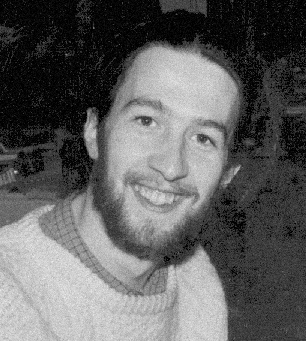
\includegraphics[width=\linewidth]{test_img/noise2.png}
      \subcaption{Original Image}
    \end{subfigure}
    \begin{subfigure}{0.49\textwidth}
      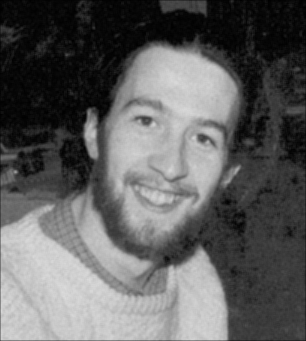
\includegraphics[width=\linewidth]{output/noise2_q1_K3P1.png}
    \subcaption{Kernel = 3}
    \end{subfigure}

    \begin{subfigure}{0.49\textwidth}
      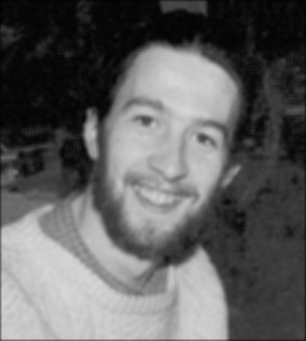
\includegraphics[width=\linewidth]{output/noise2_q1_K5P2.png}
    \subcaption{Kernel = 5}
    \end{subfigure}
    \begin{subfigure}{0.49\textwidth}
      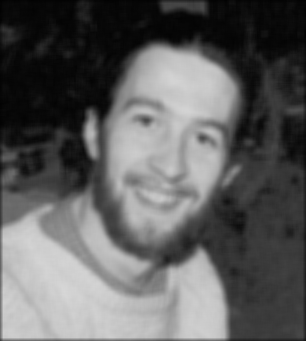
\includegraphics[width=\linewidth]{output/noise2_q1_K7P3.png}
    \subcaption{Kernel = 7}
    \end{subfigure}

  \caption{Comparison of noise2.png using Mean filter on different kernel size}
  \end{minipage}

\end{figure}
\begin{figure}[!htb]
  \begin{minipage}{\linewidth}
    \centering
    \begin{subfigure}{1\textwidth}
      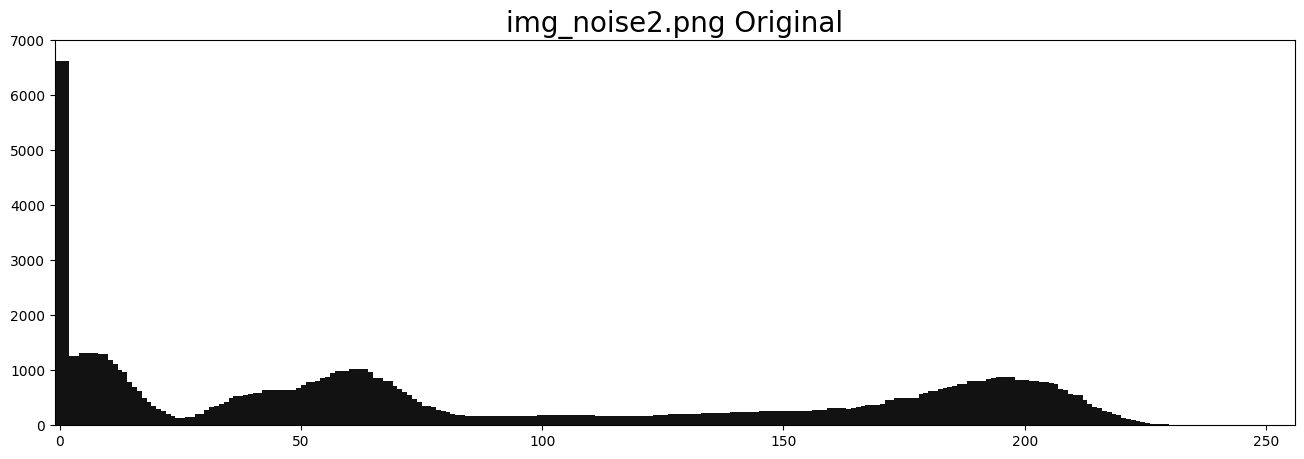
\includegraphics[height=5.3cm]{result_img/noise2_his.png}
      \subcaption{Original Image}
    \end{subfigure}
    \begin{subfigure}{1\textwidth}
      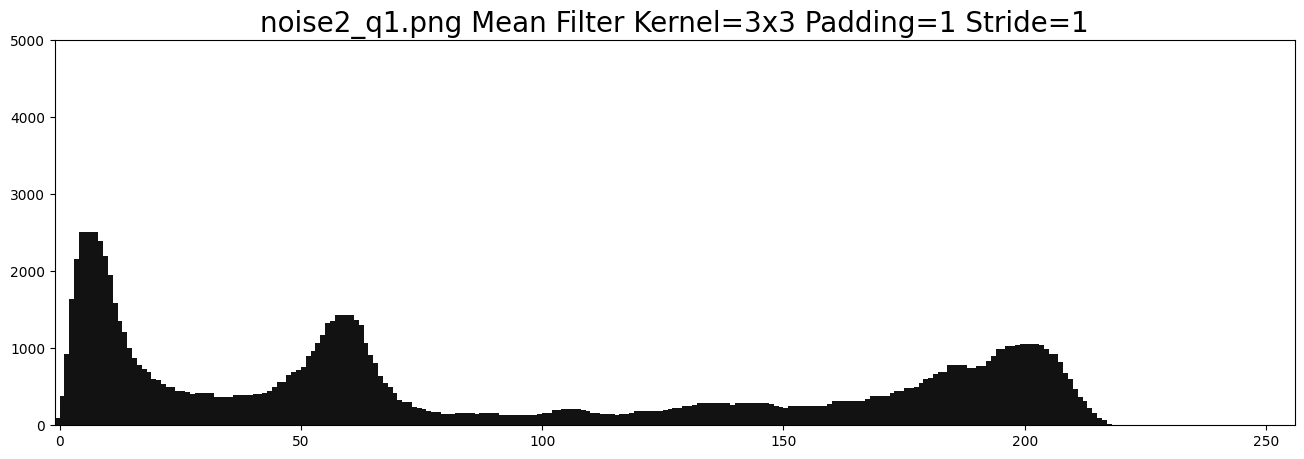
\includegraphics[height=5.3cm]{output/noise2_q1_K3P1_his.png}
    \subcaption{Kernel = 3}
    \end{subfigure}

    \begin{subfigure}{1\textwidth}
      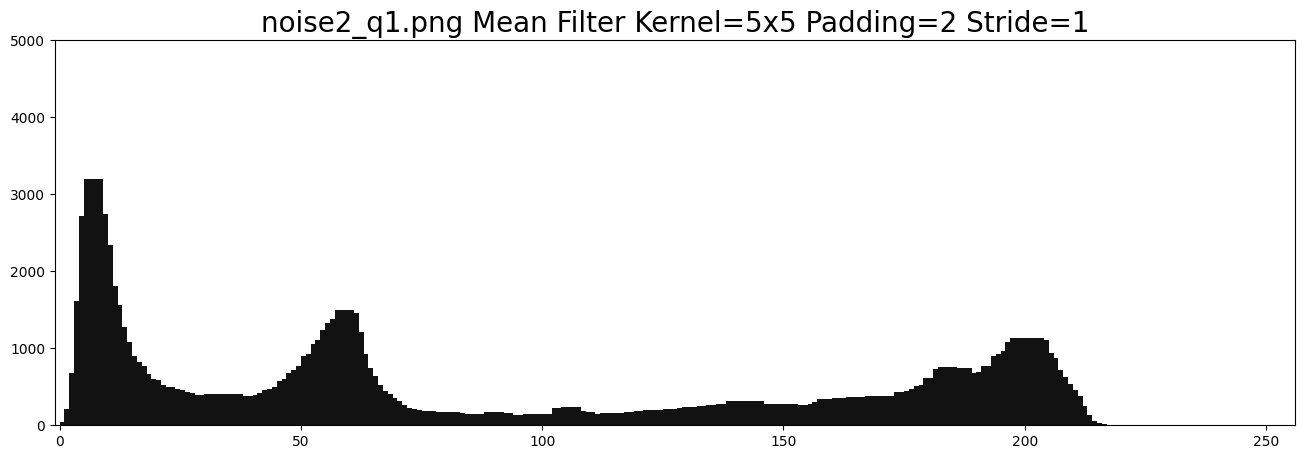
\includegraphics[height=5.3cm]{output/noise2_q1_K5P2_his.png}
    \subcaption{Kernel = 5}
    \end{subfigure}
    \begin{subfigure}{1\textwidth}
      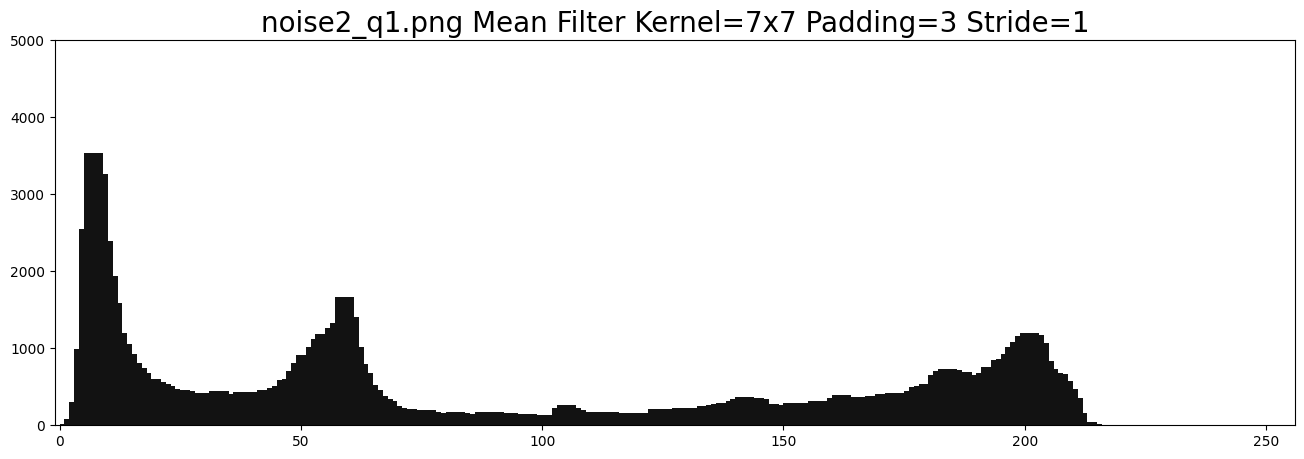
\includegraphics[height=5.3cm]{output/noise2_q1_K7P3_his.png}
    \subcaption{Kernel = 7}
    \end{subfigure}
    
  \caption{Comparison of Histogram of noise2.png using Mean filter using different kernel size}
\label{fig:n2-mean-hist}
\end{minipage}
\end{figure}
\clearpage


\subsection{Kernel size affect in Median Filter}
\paragraph*{}
Since the Median filter relies on median, which uses the data that placed in the middle of all. It means that outliers hardly affect the output since it considers place of data rather than value. It makes this filter tolerants to salt and pepper noise. Selecting higher or lower number of kernel size not affects that much on the result. The only case that size of kernel affects the result is when the noise is burst noise.
\paragraph*{}One of effect that need to be mentioned about Median filter is the Median filter reduce the detail. Since the result not relies on the individual input value. Fluctuation of inputs (which is considered `detail') lost during this process. Moreover, the larger kernel size, the more loss in detail.
\paragraph*{}Median filter sharpen the histogram curve, especially around the high dense area as shown in Figure~\ref{fig:n2-median-hist}.

\begin{figure}[!htb]
  \begin{minipage}{\linewidth}
    \centering
    \begin{subfigure}{0.49\textwidth}
      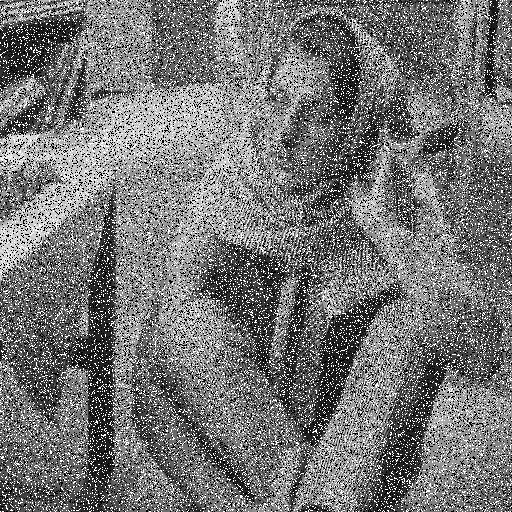
\includegraphics[width=\linewidth]{test_img/noise1.png}
      \subcaption{Original Image}
    \end{subfigure}
    \begin{subfigure}{0.49\textwidth}
      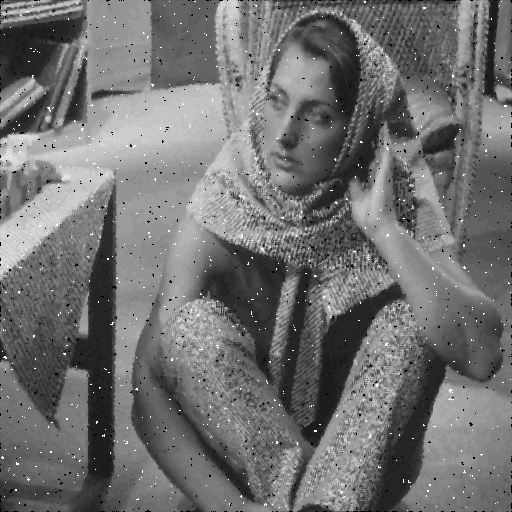
\includegraphics[width=\linewidth]{output/noise1_q2_K3P1.png}
    \subcaption{Kernel = 3}
    \end{subfigure}

    \begin{subfigure}{0.49\textwidth}
      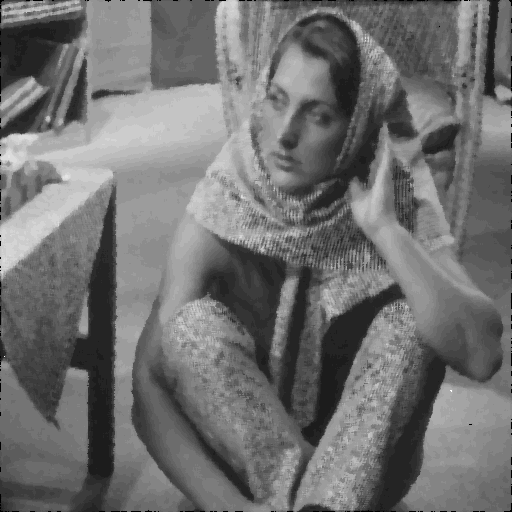
\includegraphics[width=\linewidth]{output/noise1_q2_K5P2.png}
    \subcaption{Kernel = 5}
    \end{subfigure}
    \begin{subfigure}{0.49\textwidth}
      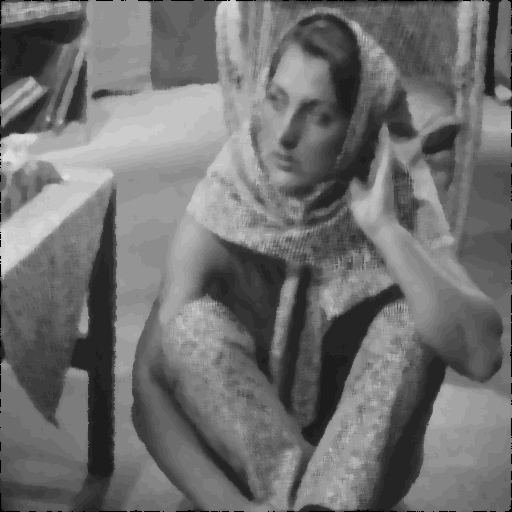
\includegraphics[width=\linewidth]{output/noise1_q2_K7P3.png}
    \subcaption{Kernel = 7}
    \end{subfigure}

  \caption{Comparison of noise1.png using Mean filter on different kernel size}
  \end{minipage}

\end{figure}
\begin{figure}[!htb]
  \begin{minipage}{\linewidth}
    \centering
    \begin{subfigure}{1\textwidth}
      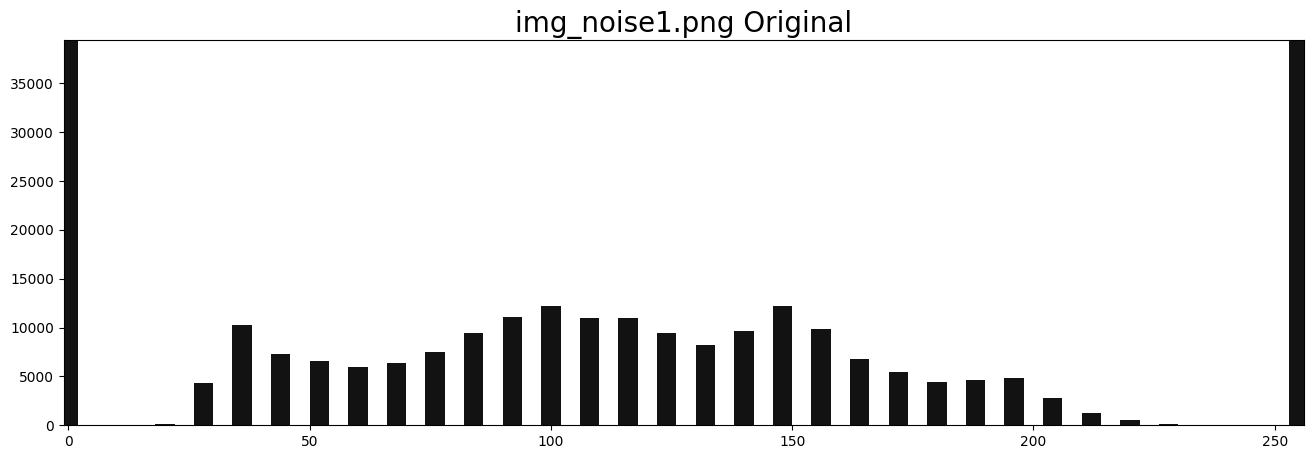
\includegraphics[height=5.3cm]{result_img/noise1_his.png}
      \subcaption{Original Image}
    \end{subfigure}
    \begin{subfigure}{1\textwidth}
      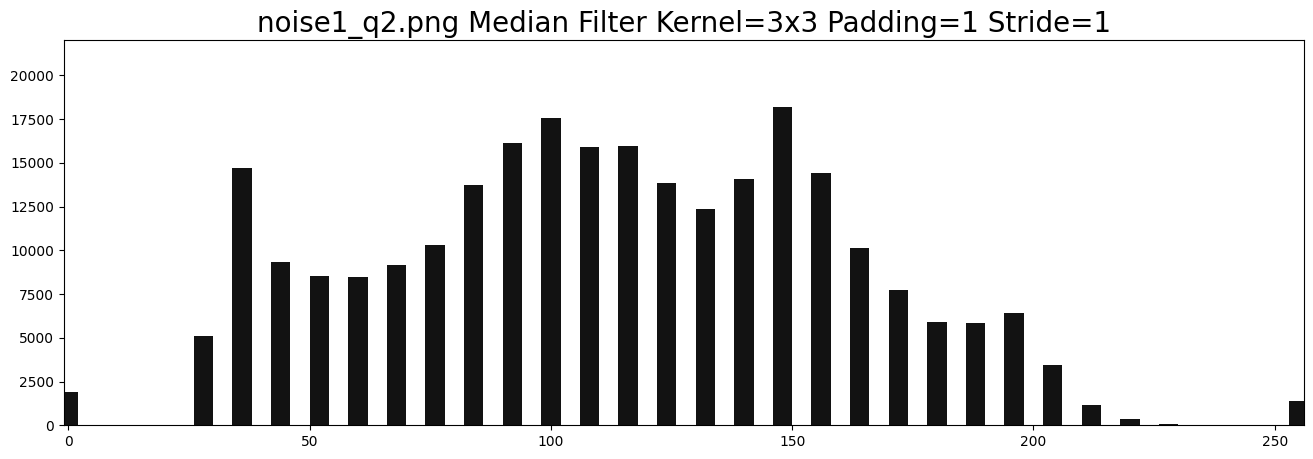
\includegraphics[height=5.3cm]{output/noise1_q2_K3P1_his.png}
    \subcaption{Kernel = 3}
    \end{subfigure}

    \begin{subfigure}{1\textwidth}
      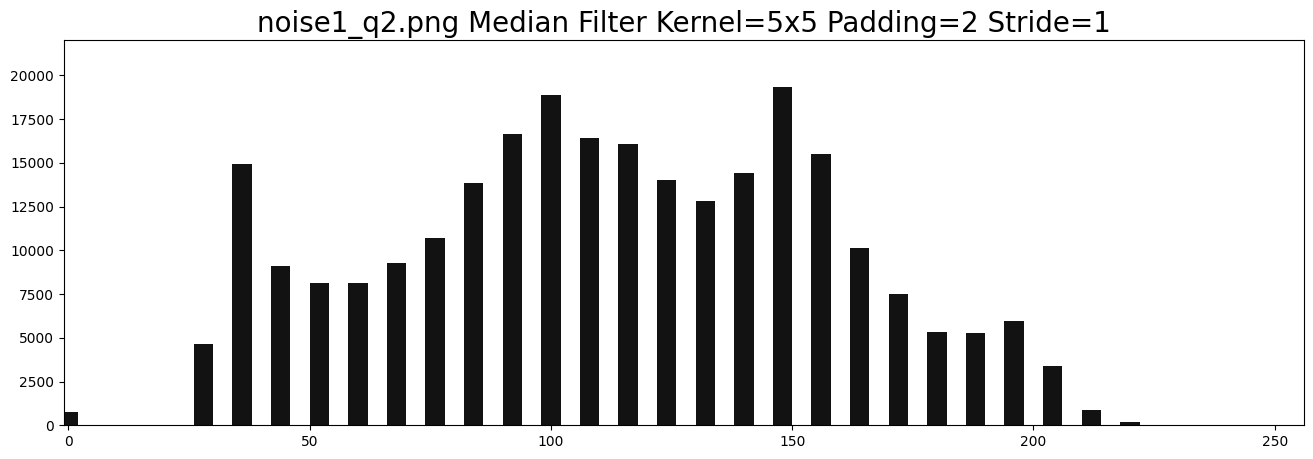
\includegraphics[height=5.3cm]{output/noise1_q2_K5P2_his.png}
    \subcaption{Kernel = 5}
    \end{subfigure}
    \begin{subfigure}{1\textwidth}
      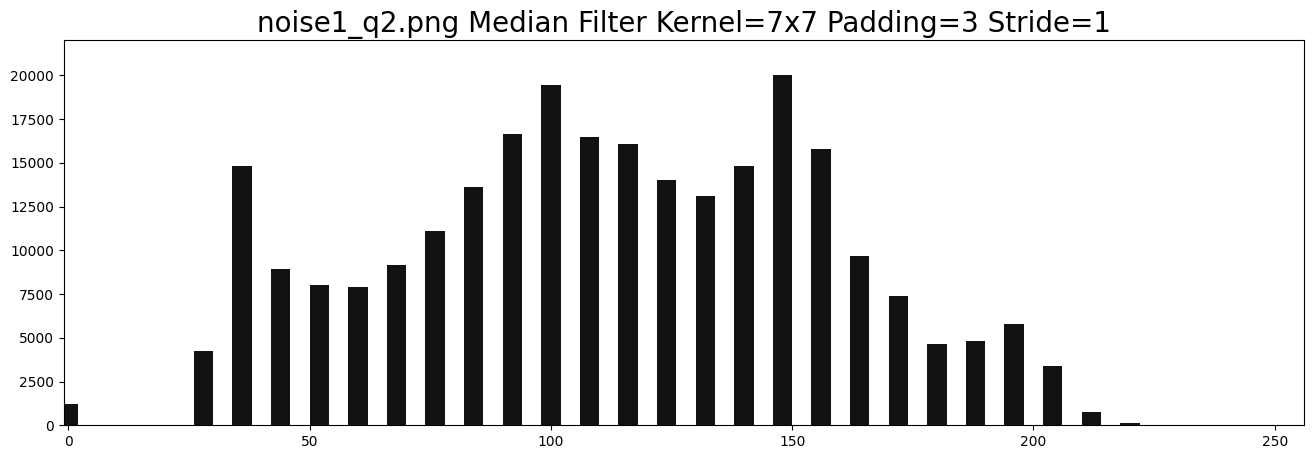
\includegraphics[height=5.3cm]{output/noise1_q2_K7P3_his.png}
    \subcaption{Kernel = 7}
    \end{subfigure}
    
  \caption{Comparison of Histogram of noise1.png using Mean filter on different kernel size}
\label{fig:n1-median-hist}
\end{minipage}
\end{figure}
\begin{figure}[!htb]
  \begin{minipage}{\linewidth}
    \centering
    \begin{subfigure}{0.49\textwidth}
      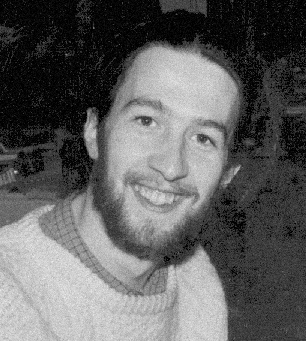
\includegraphics[width=\linewidth]{test_img/noise2.png}
      \subcaption{Original Image}
    \end{subfigure}
    \begin{subfigure}{0.49\textwidth}
      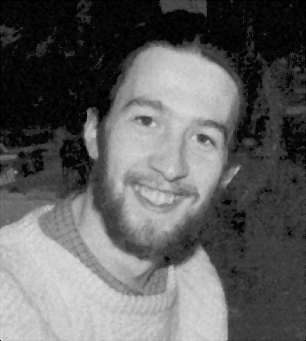
\includegraphics[width=\linewidth]{output/noise2_q2_K3P1.png}
    \subcaption{Kernel = 3}
    \end{subfigure}

    \begin{subfigure}{0.49\textwidth}
      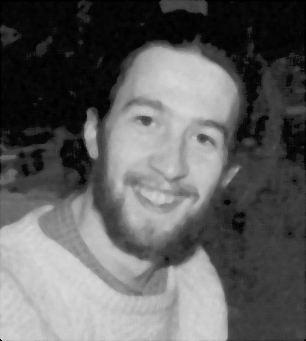
\includegraphics[width=\linewidth]{output/noise2_q2_K5P2.png}
    \subcaption{Kernel = 5}
    \end{subfigure}
    \begin{subfigure}{0.49\textwidth}
      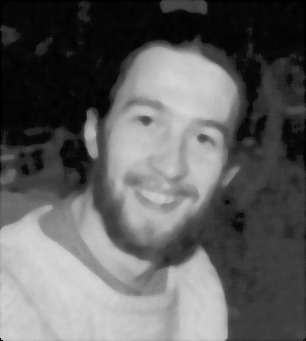
\includegraphics[width=\linewidth]{output/noise2_q2_K7P3.png}
    \subcaption{Kernel = 7}
    \end{subfigure}

  \caption{Comparison of noise2.png using Mean filter on different kernel size}
  \end{minipage}

\end{figure}
\begin{figure}[!htb]
  \begin{minipage}{\linewidth}
    \centering
    \begin{subfigure}{1\textwidth}
      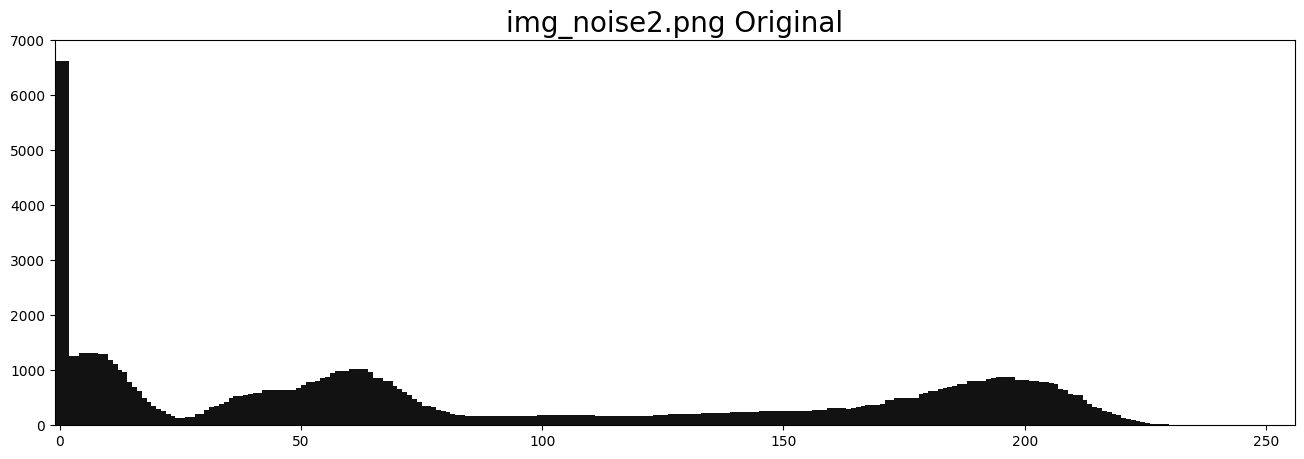
\includegraphics[height=5.3cm]{result_img/noise2_his.png}
      \subcaption{Original Image}
    \end{subfigure}
    \begin{subfigure}{1\textwidth}
      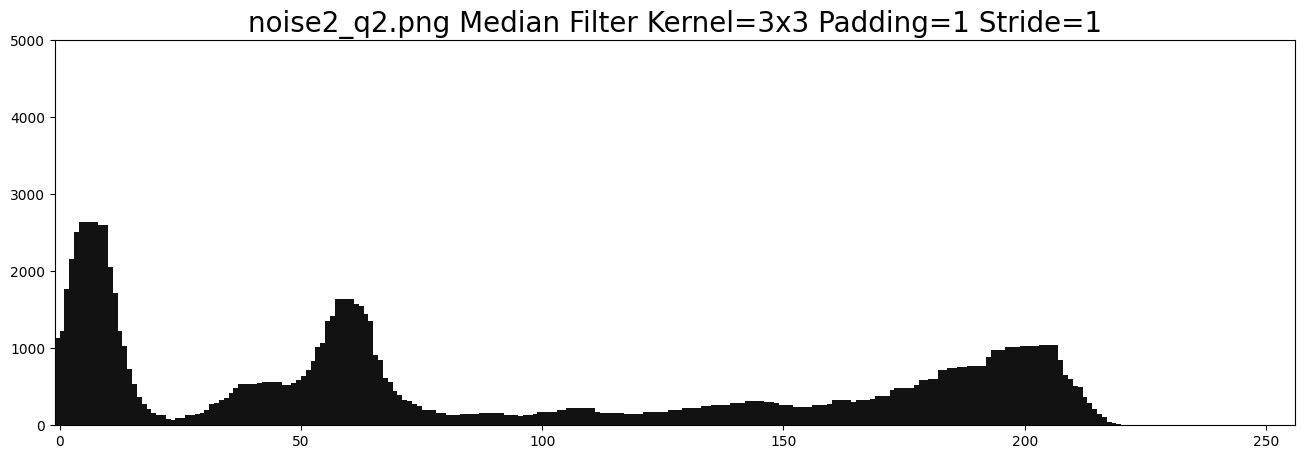
\includegraphics[height=5.3cm]{output/noise2_q2_K3P1_his.png}
    \subcaption{Kernel = 3}
    \end{subfigure}

    \begin{subfigure}{1\textwidth}
      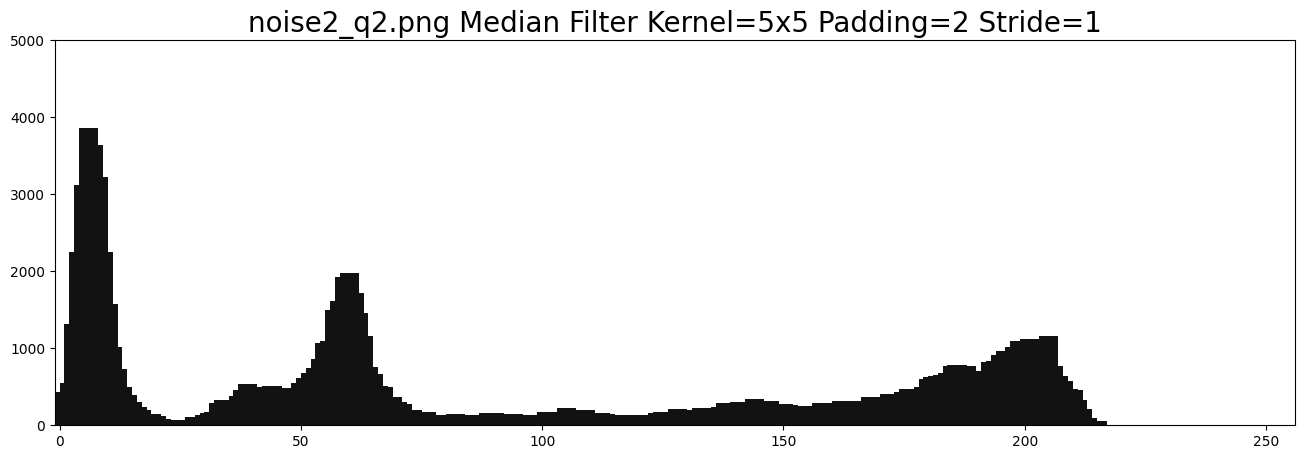
\includegraphics[height=5.3cm]{output/noise2_q2_K5P2_his.png}
    \subcaption{Kernel = 5}
    \end{subfigure}
    \begin{subfigure}{1\textwidth}
      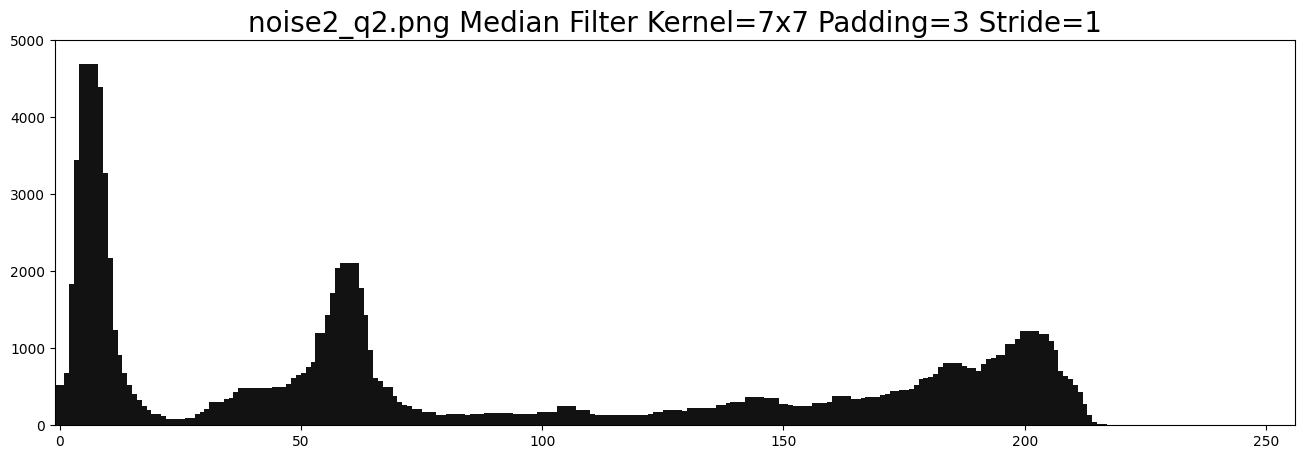
\includegraphics[height=5.3cm]{output/noise2_q2_K7P3_his.png}
    \subcaption{Kernel = 7}
    \end{subfigure}
    
  \caption{Comparison of Histogram of noise2.png using Mean filter using different kernel size}
\label{fig:n2-median-hist}
\end{minipage}
\end{figure}
\clearpage
\subsection{Choosing Filter}
\paragraph*{}Please be reminded that there is no single, complete formula that yields the best
result. For this case, prior knowledge about the noise appears in the image can play a vital role in order to choose the appropriate filter. If the system observed tends to have a salt and pepper noise, using Median filter might give a better result. While the Mean filter is still considered a safe decision, since the real environment tends to have a gaussian noise which can be attenuated by the Mean filter.
\paragraph*{}Sequentially Applying filter might improve the result since each filter has it own advantages.

\paragraph*{}Another consideration point is computation complexity. Since Median filter is not a calculation but sorting. Sorting algorithm used affects the performance and complexity directly. For the optimum solution, it need to weighted as same as the result quality.

\appendix
\chapter{Git Repository}

\verb|Git Repository: chinatip-l/computer-vision-lab-fall-2023| \\
URL: \url{https://github.com/chinatip-l/computer-vision-lab-fall-2023}

\chapter{Source Code: main.cpp}
\begin{lstlisting}
#include <stdio.h>
#include <opencv2/opencv.hpp>
#include <unistd.h>
#include <string.h>
#include "include/func.hpp"

#define MAX_LEN 250
#define BASE_PATH "/home/chinatip/work/computer_vision/homework2"
#define SRC_PATH "test_img"
#define OUT_PATH "output"

// define file name, can uncomment to select the input
#define FILENAME "noise1"
// #define FILENAME "noise2"
#define MEAN_FILT_SUFX "q1"
#define MEDIAN_FILT_SUFX "q2"
#define KER_INFO_3 "K3P1"
#define KER_INFO_5 "K5P2"
#define KER_INFO_7 "K7P3"
#define EXT "png"

using namespace cv;

Mat canvas;

void appendImgToCanvas(Mat);

int main(int argc, char **argv)
{

    Mat og_img;
    char og_file[MAX_LEN] = "", out_file[MAX_LEN] = "";
    snprintf(og_file, MAX_LEN, "%s/%s/%s.%s", BASE_PATH, SRC_PATH, FILENAME, EXT);

    og_img = imread(og_file);

    if (!og_img.data)
    {
        printf("No image data \n");
        return -1;
    }
    else
    {
        printf("Original Img Size: w x h %d x %d\n", og_img.cols, og_img.rows);
    }

    appendImgToCanvas(og_img);

    Mat res_img;
    res_img = applyMedianFilter(og_img,3,1,1);
    printf("Median Filter Img Size: w x h %d x %d\n", res_img.cols, res_img.rows);
    snprintf(out_file, MAX_LEN, "%s/%s/%s_%s.%s", BASE_PATH, OUT_PATH, FILENAME, MEDIAN_FILT_SUFX, EXT);
    imwrite(out_file, res_img);
    snprintf(out_file, MAX_LEN, "%s/%s/%s_%s_%s.%s", BASE_PATH, OUT_PATH, FILENAME, MEDIAN_FILT_SUFX,KER_INFO_3, EXT);
    imwrite(out_file, res_img);
    appendImgToCanvas(res_img);

    res_img = applyMedianFilter(og_img,5,2,1);
    printf("Median Filter Img Size: w x h %d x %d\n", res_img.cols, res_img.rows);
    snprintf(out_file, MAX_LEN, "%s/%s/%s_%s_%s.%s", BASE_PATH, OUT_PATH, FILENAME, MEDIAN_FILT_SUFX,KER_INFO_5, EXT);
    imwrite(out_file, res_img);
    appendImgToCanvas(res_img);

    res_img = applyMedianFilter(og_img,7,3,1);
    printf("Median Filter Img Size: w x h %d x %d\n", res_img.cols, res_img.rows);
    snprintf(out_file, MAX_LEN, "%s/%s/%s_%s_%s.%s", BASE_PATH, OUT_PATH, FILENAME, MEDIAN_FILT_SUFX,KER_INFO_7, EXT);
    imwrite(out_file, res_img);
    appendImgToCanvas(res_img);

    namedWindow("Original", WINDOW_AUTOSIZE);
    
    imshow("Original", canvas);
    waitKey(0);
    return 0;
}

void appendImgToCanvas(Mat img)
{
    if (canvas.empty())
    {
        canvas = img;
    }
    else
    {
        Size s(canvas.cols + img.cols + 5, canvas.rows>img.rows?canvas.rows:img.rows);
        size_t old_w = canvas.cols;
        copyMakeBorder(canvas, canvas, 0, 0, 0, img.cols + 5, BORDER_CONSTANT, Scalar(0, 0, 0, 0));
        img.copyTo(canvas(Rect(old_w + 5, 0, img.cols, img.rows)));
    }
}

  

\end{lstlisting}

\chapter{Source Code: func.hpp}
\begin{lstlisting}
#ifndef _FUNC_H_
#define _FUNC_H_

#include <opencv2/opencv.hpp>
#include <vector>

using namespace cv;

Mat applyMeanFilter(Mat,int,int,int);
Mat applyMedianFilter(Mat,int,int,int);
static std::vector<int32_t> sort(std::vector<int32_t>);

#endif
\end{lstlisting}

\chapter{Source Code: func.cpp}
\begin{lstlisting}
#include "include/func.hpp"
#include <vector>

typedef struct node
{
  int32_t val;
  struct node* next;
  bool is_term;
}node_t;

node_t END={.val=0,.next=nullptr,.is_term=true};


Mat applyMeanFilter (Mat img, int kernel_size, int padding, int stride)
{
  // calculate kernel offset ie. number of pixel before and 
  // after since the target pixel will be the center of 
  // matrix,
  // in order to get the neighbour pixel with size of kernel
  // size, offset will be applied for both before, and after
  // the target pixel
  // example
  // width = 5 => offset = (int)5/2 = 2;
  // px   ... k   n-offset    ... n   ... n+offset    k
  int ker_x_offset = kernel_size / 2;
  int ker_y_offset = kernel_size / 2;

  // get kernel size
  int ker_w = kernel_size;
  int ker_h = kernel_size;

  // calculate output image size
  int out_w = ((img.cols + (2 * padding) - kernel_size) / stride) + 1;
  int out_h = ((img.rows + (2 * padding) - kernel_size) / stride) + 1;

  // create intermediate buffer and add padding, size is 
  // w+(2*padding),h+(2*padding) then copy the content 
  // of image to the buffer
  Mat padded;
  padded = Mat::zeros(img.rows + (2 * padding), img.cols + (2 * padding), CV_32SC3);
  for (int j = 0; j < img.rows; j++)
  {
      for (int i = 0; i < img.cols; i++)
      {
          padded.at<Vec3i>(j+padding,i+padding)=img.at<Vec3b>(j,i);
      }
  }
  
  // create output buffer with calculated output size
  // data type need to be vector of signed int 32 bit
  // in case negative data is possible, this can help
  // preserve information through the convolution process
  // and rasterise to 8 bit at the last step
  Mat img_res = Mat::zeros(out_h, out_w, CV_32SC3);
  Vec3i res(0, 0, 0);
  Point2i start=Point2i(0,0);

  // iterate over the size of input image
  for (int out_j = 0; out_j < out_h; out_j++)
  {
      for (int out_i = 0; out_i < out_w; out_i++)
      {
          
          // calculate the start point to slice a windowed from 
          // the padded buffer
          start.x=(out_i*stride)+padding-ker_x_offset;
          start.y=(out_j*stride)+padding-ker_x_offset;

          // get windowed matrix from the padded buffer with 
          // the size of kernel size, and target pixel is in
          // the center of windowed matrix
          Mat windowed = padded(Rect(start.x, start.y, ker_w, ker_h));
          res = Vec3i(0, 0, 0);


          // item-wise multiply windowed matrix with kernel 
          // matrix and summarise 
          for (int ker_j = 0; ker_j < kernel_size; ker_j++)
          {
              for (int ker_i = 0; ker_i < kernel_size; ker_i++)
              {
                  Vec3b t = windowed.at<Vec3i>(ker_i, ker_j);
                  
                  // add to buffer
                  res+=t;
              }
          }

          for (int c = 0; c < 3; c++)
          {
              // divide by the number of elements
              res[c] /= (kernel_size*kernel_size);
          }

          // write to output buffer
          img_res.at<Vec3i>(out_j,out_i) = res;
          
      }
  }

  // return the output image
  return img_res;
}

Mat applyMedianFilter (Mat img, int kernel_size, int padding, int stride)
{
  // calculate kernel offset ie. number of pixel before and 
  // after since the target pixel will be the center of 
  // matrix,
  // in order to get the neighbour pixel with size of kernel
  // size, offset will be applied for both before, and after
  // the target pixel
  // example
  // width = 5 => offset = (int)5/2 = 2;
  // px   ... k   n-offset    ... n   ... n+offset    k
  int ker_x_offset = kernel_size / 2;
  int ker_y_offset = kernel_size / 2;

  // get kernel size
  int ker_w = kernel_size;
  int ker_h = kernel_size;

  // calculate output image size
  int out_w = ((img.cols + (2 * padding) - kernel_size) / stride) + 1;
  int out_h = ((img.rows + (2 * padding) - kernel_size) / stride) + 1;

  // create intermediate buffer and add padding, size is 
  // w+(2*padding),h+(2*padding) then copy the content 
  // of image to the buffer
  Mat padded;
  padded = Mat::zeros(img.rows + (2 * padding), img.cols + (2 * padding), CV_32SC3);
  for (int j = 0; j < img.rows; j++)
  {
      for (int i = 0; i < img.cols; i++)
      {
          padded.at<Vec3i>(j+padding,i+padding)=img.at<Vec3b>(j,i);
      }
  }
  
  // create output buffer with calculated output size
  // data type need to be vector of signed int 32 bit
  // in case negative data is possible, this can help
  // preserve information through the convolution process
  // and rasterise to 8 bit at the last step
  Mat img_res = Mat::zeros(out_h, out_w, CV_32SC3);
  Vec3i res(0, 0, 0);
  Point2i start=Point2i(0,0);

  // iterate over the size of input image
  for (int out_j = 0; out_j < out_h; out_j++)
  {
      for (int out_i = 0; out_i < out_w; out_i++)
      {

          
          // calculate the start point to slice a windowed from 
          // the padded buffer
          start.x=(out_i*stride)+padding-ker_x_offset;
          start.y=(out_j*stride)+padding-ker_x_offset;

          // get windowed matrix from the padded buffer with 
          // the size of kernel size, and target pixel is in
          // the center of windowed matrix
          Mat windowed = padded(Rect(start.x, start.y, ker_w, ker_h));
          res = Vec3i(0, 0, 0);

          // create buffer lists for each channel
          std::vector<int32_t> b,g,r;


          // item-wise split channel data             
          for (int ker_j = 0; ker_j < kernel_size; ker_j++)
          {
              for (int ker_i = 0; ker_i < kernel_size; ker_i++)
              {
                  Vec3b t = windowed.at<Vec3i>(ker_i, ker_j);
              
                  // add each channel to its buffer list
                  b.push_back(t[0]);
                  g.push_back(t[1]);
                  r.push_back(t[2]);
              }
          }
          
          // apply sort function to each channel
          b=sort(b);
          r=sort(r);
          g=sort(g);

          // get the median ie. the middle item of the list
          // as a representative for each window
          int idx=b.size()/2;
          res[0]=b.at(idx);
          res[1]=g.at(idx);
          res[2]=r.at(idx);

          // write to output buffer
          img_res.at<Vec3i>(out_j,out_i) = res;
          
      }
  }

  // return the output image
  return img_res;
}

std::vector<int32_t> sort(std::vector<int32_t> list){
  // using insertion sort

  // initialise head of the list, and point to the end
  node_t head={.next=&END};
  node_t* cur;
  node_t* tmp;

  // for each item in list
  for(int i=0;i<list.size();i++){

      //first, set current node to head
      cur=&head;

      //create new node with current data
      tmp=(node_t*)malloc(sizeof(node_t));
      tmp->val=list.at(i);

      // traverse through linked list
      while(true){
          if(cur->next->is_term==true){
              // if reach end node, insert new node as
              // the last node of the linked list
              tmp->next=cur->next;
              cur->next=tmp;
              break;
          }else if(tmp->val<=cur->next->val){
              // if not the last node, compare value with
              // the next node, if lesser or equal to the 
              // next node, put new node at the current 
              // position and point to the next
              tmp->next=cur->next;
              cur->next=tmp;
              break;
          }
          // else, continue to next node
          cur=cur->next;
      }
  }

  //after sort, traverse through linked list and put back to vector
  cur=&head;
  cur=cur->next;
  std::vector<int32_t> res;
  while(!cur->is_term){
      res.push_back(cur->val);
      tmp=cur;
      cur=cur->next;
      free(tmp);
  }
  return res;
  
}

\end{lstlisting}

\chapter{Source Code: graph.py}
\begin{lstlisting}
import matplotlib.pyplot as plt
import cv2
import numpy as np
import re
import glob
FILE_PATH="output"
files=[f for f in glob.glob(f"{FILE_PATH}/*.png") if re.findall(r'his', f)==[]]

for f in files:
    
    n=re.split("\.|/|_|K|P",f)
    print(n)
    if len(n)==7:
        q= "Mean" if n[2]=='q1' else "Median" 
        k=int(n[4])
        p=int(n[5])
    else:
        q="Original"
    image = cv2.imread(f)
    print(type(image))
    print(image.dtype)
    print(image.shape)
    b=[0]*256
    for i in image:
        for j in i:
            b[j[0]]+=1

    
    plt.figure(figsize=(16, 5), dpi=100)
    plt.xlim([-1,256])
    if max(b)<5000:
        plt.ylim([0,5000])
    else:
        plt.ylim([0,22000])
    sn=re.split("\.|/",f)
    print(sn)
    if(q!="Original"):
        plt.title(f"{n[1]}_{n[2]}.png {q} Filter Kernel={k}x{k} Padding={p} Stride=1", fontsize=20)
    else:
        plt.title(f"{n[1]}_{n[2]}.png {q}", fontsize=20)
        if max(b)<8000:
            plt.ylim([0,7000])
        else:
            plt.ylim([0,max(b)])
    plt.bar(range(0,256),b,width=4, color='#121212')
    
    plt.savefig(f"{sn[0]}/{sn[1]}_his.{sn[2]}",bbox_inches='tight')

\end{lstlisting}

\chapter{Result Images}
\begin{figure}[!htb]
  \centering
  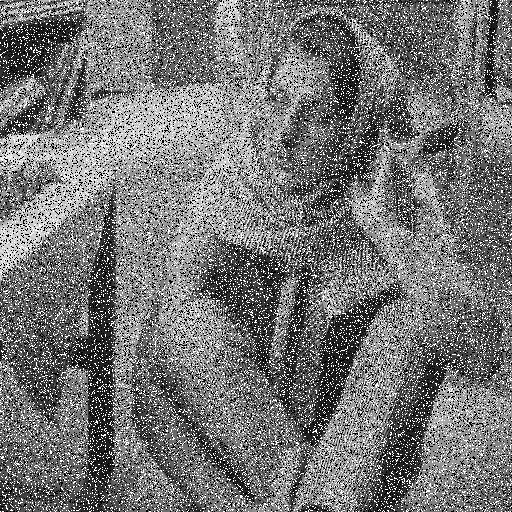
\includegraphics[width=1\linewidth]{test_img/noise1.png}
  \caption{Original noise1}
  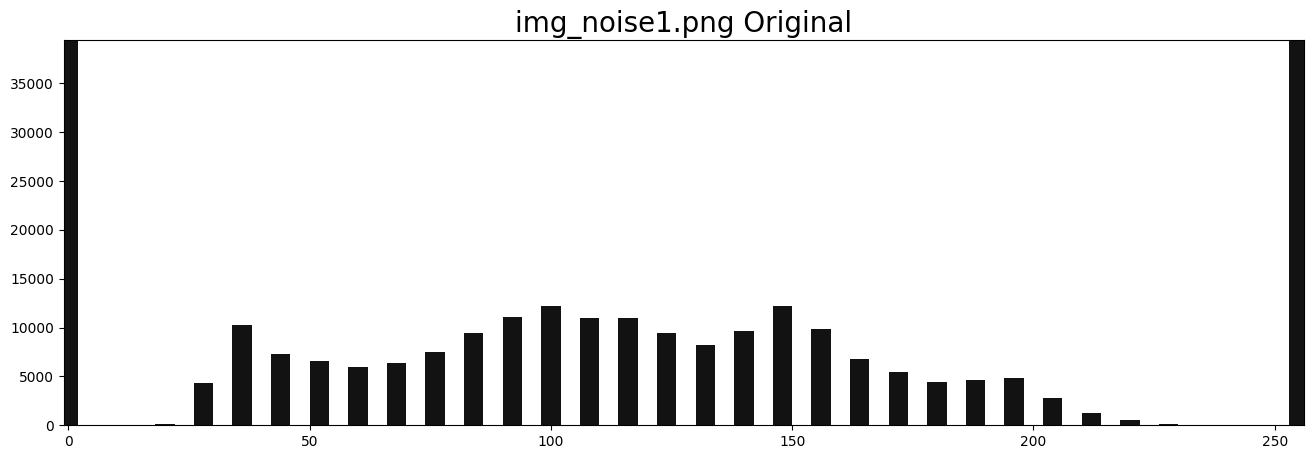
\includegraphics[width=1\linewidth]{result_img/noise1_his.png}
  \caption{Original noise1 Histogram}
\end{figure}
\begin{figure}[!htb]
  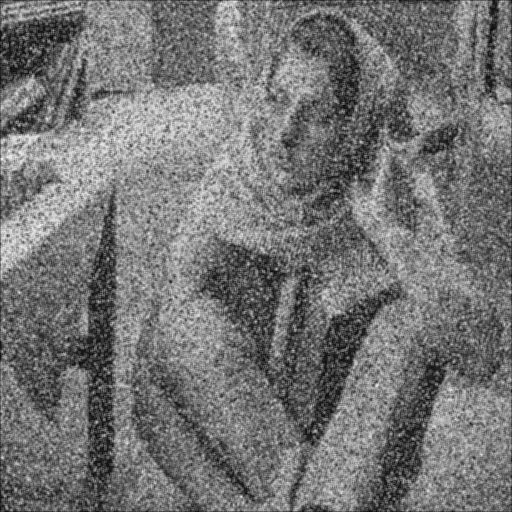
\includegraphics[width=1\linewidth]{output/noise1_q1_K3P1.png}
  \caption{Mean Filter noise1 K=3 Output}
  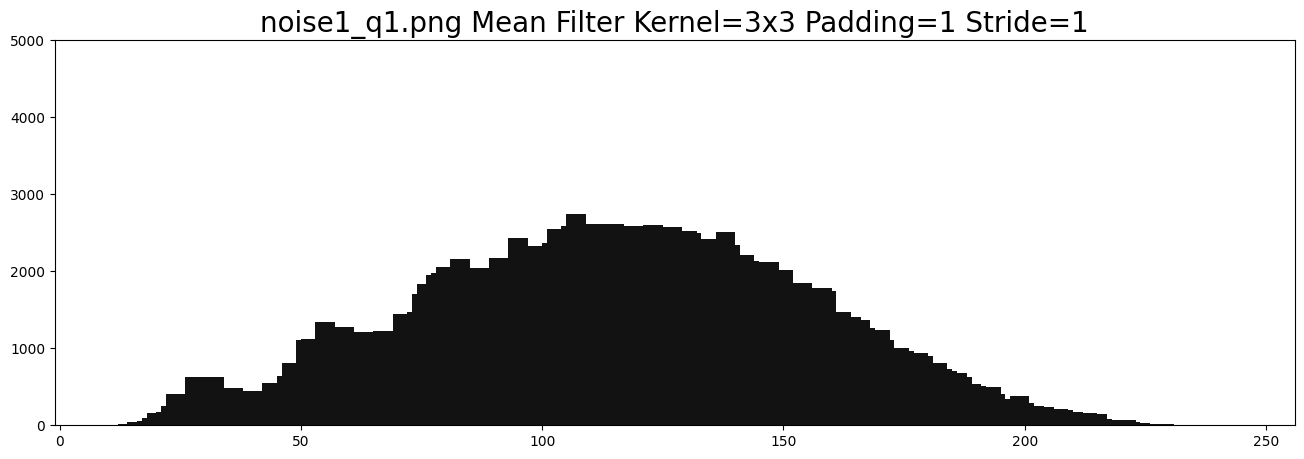
\includegraphics[width=1\linewidth]{output/noise1_q1_K3P1_his.png}
  \caption{Mean Filter noise1 K=3 Histogram}
\end{figure}
\begin{figure}[!htb]
  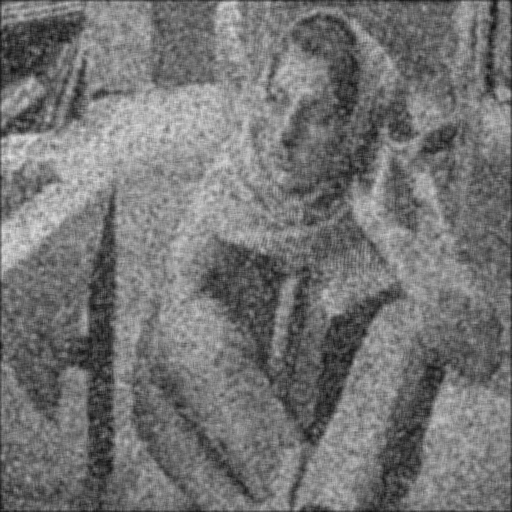
\includegraphics[width=1\linewidth]{output/noise1_q1_K5P2.png}
  \caption{Mean Filter noise1 K=5 Output}
  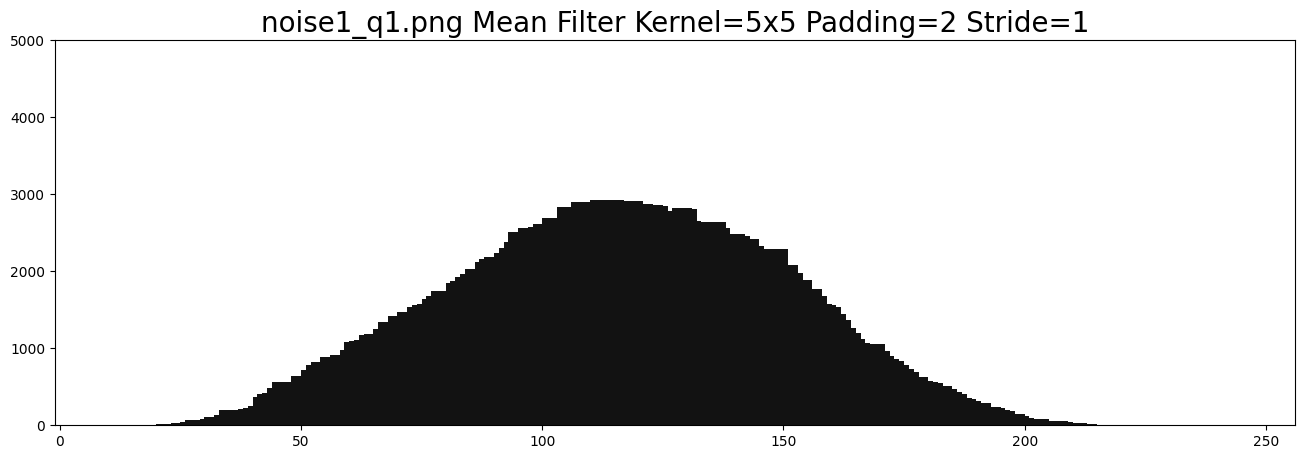
\includegraphics[width=1\linewidth]{output/noise1_q1_K5P2_his.png}
  \caption{Mean Filter noise1 K=5 Histogram}
\end{figure}
\begin{figure}[!htb]
  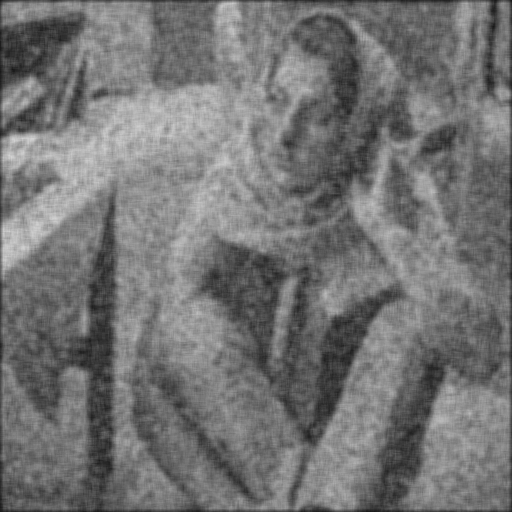
\includegraphics[width=1\linewidth]{output/noise1_q1_K7P3.png}
  \caption{Mean Filter noise1 K=7 Output}
  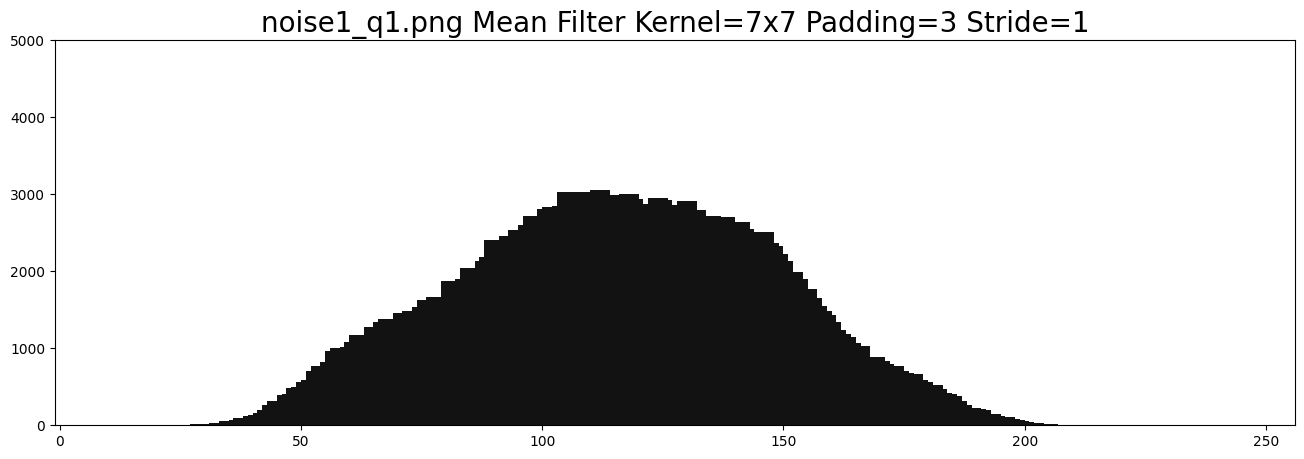
\includegraphics[width=1\linewidth]{output/noise1_q1_K7P3_his.png}
  \caption{Mean Filter noise1 K=7 Histogram}
\end{figure}
\begin{figure}[!htb]
  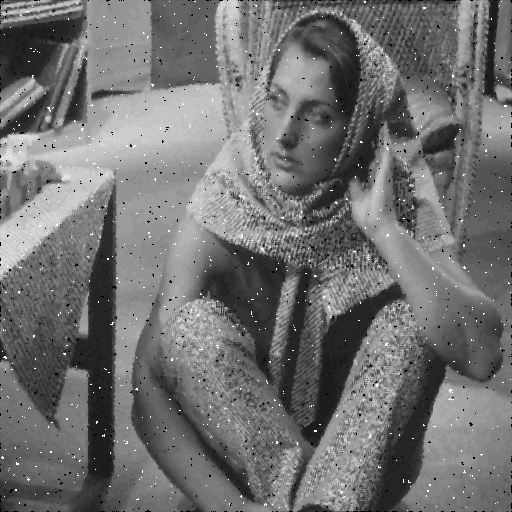
\includegraphics[width=1\linewidth]{output/noise1_q2_K3P1.png}
  \caption{Median Filter noise1 K=3 Output}
  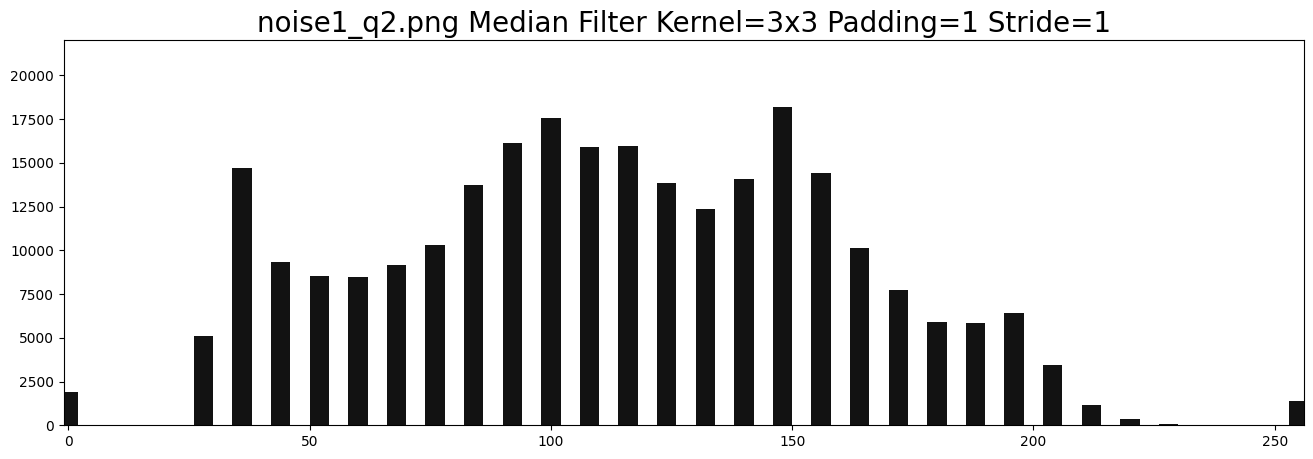
\includegraphics[width=1\linewidth]{output/noise1_q2_K3P1_his.png}
  \caption{Median Filter noise1 K=3 Histogram}
\end{figure}
\begin{figure}[!htb]
  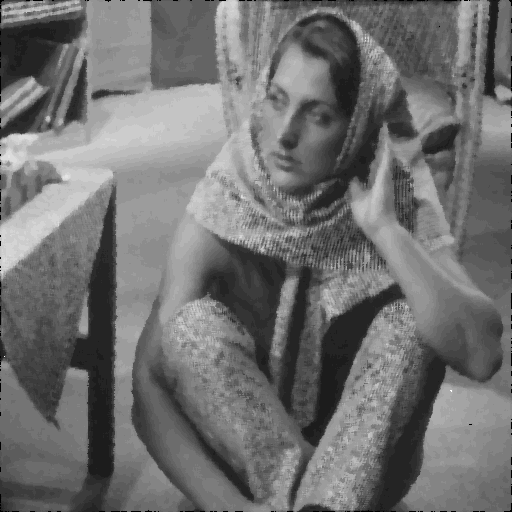
\includegraphics[width=1\linewidth]{output/noise1_q2_K5P2.png}
  \caption{Median Filter noise1 K=5 Output}
  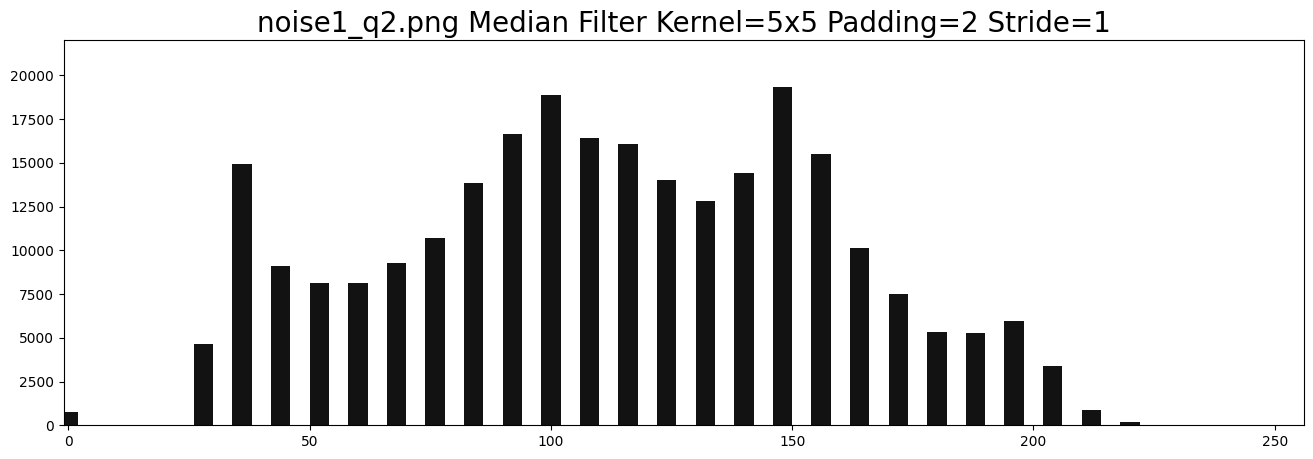
\includegraphics[width=1\linewidth]{output/noise1_q2_K5P2_his.png}
  \caption{Median Filter noise1 K=5 Histogram}
\end{figure}
\begin{figure}[!htb]
  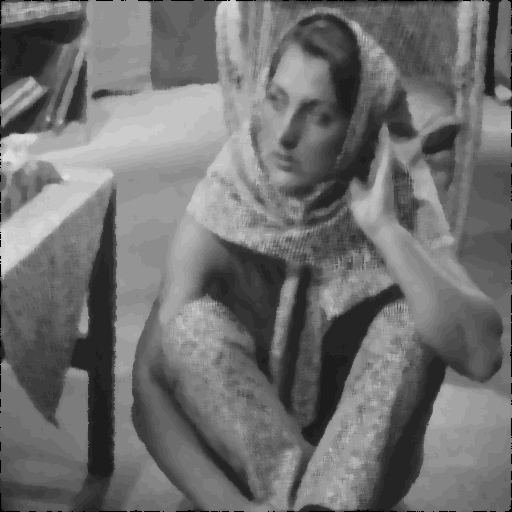
\includegraphics[width=1\linewidth]{output/noise1_q2_K7P3.png}
  \caption{Median Filter noise1 K=7 Output}
  \includegraphics[width=1\linewidth]{output/noise1_q2_K7P3_his.png}
  \caption{Median Filter noise1 K=7 Histogram}
\end{figure}

\begin{figure}[!htb]
  \centering
  \includegraphics[width=1\linewidth]{test_img/noise2.png}
  \caption{Original noise2}
  \includegraphics[width=1\linewidth]{result_img/noise2_his.png}
  \caption{Original noise2 Histogram}
\end{figure}
\begin{figure}[!htb]
  \includegraphics[width=1\linewidth]{output/noise2_q1_K3P1.png}
  \caption{Mean Filter noise2 K=3 Output}
  \includegraphics[width=1\linewidth]{output/noise2_q1_K3P1_his.png}
  \caption{Mean Filter noise2 K=3 Histogram}
\end{figure}
\begin{figure}[!htb]
  \includegraphics[width=1\linewidth]{output/noise2_q1_K5P2.png}
  \caption{Mean Filter noise2 K=5 Output}
  \includegraphics[width=1\linewidth]{output/noise2_q1_K5P2_his.png}
  \caption{Mean Filter noise2 K=5 Histogram}
\end{figure}
\begin{figure}[!htb]
  \includegraphics[width=1\linewidth]{output/noise2_q1_K7P3.png}
  \caption{Mean Filter noise2 K=7 Output}
  \includegraphics[width=1\linewidth]{output/noise2_q1_K7P3_his.png}
  \caption{Mean Filter noise2 K=7 Histogram}
\end{figure}
\begin{figure}[!htb]
  \includegraphics[width=1\linewidth]{output/noise2_q2_K3P1.png}
  \caption{Median Filter noise2 K=3 Output}
  \includegraphics[width=1\linewidth]{output/noise2_q2_K3P1_his.png}
  \caption{Median Filter noise2 K=3 Histogram}
\end{figure}
\begin{figure}[!htb]
  \includegraphics[width=1\linewidth]{output/noise2_q2_K5P2.png}
  \caption{Median Filter noise2 K=5 Output}
  \includegraphics[width=1\linewidth]{output/noise2_q2_K5P2_his.png}
  \caption{Median Filter noise2 K=5 Histogram}
\end{figure}
\begin{figure}[!htb]
  \includegraphics[width=1\linewidth]{output/noise2_q2_K7P3.png}
  \caption{Median Filter noise2 K=7 Output}
  \includegraphics[width=1\linewidth]{output/noise2_q2_K7P3_his.png}
  \caption{Median Filter noise2 K=7 Histogram}
\end{figure}
\end{document}
